\documentclass[a4paper]{article}
%\VignetteIndexEntry{Ham94: Companion to James Hamilton's "Time Series Analysis"}
\usepackage[latin9]{inputenc}
\usepackage{verbatim}
\usepackage{amsmath}
\usepackage{Sweave}
\usepackage{url}
\usepackage[unicode=true, pdfusetitle, backref=false,colorlinks=false] {hyperref}



%\providecommand*{\perispomeni}{\char126}
%\AtBeginDocument{\DeclareRobustCommand{\greektext}{%
%  \fontencoding{LGR}\selectfont\def\encodingdefault{LGR}%
%  \renewcommand{\~}{\perispomeni}%
%}}
%\DeclareRobustCommand{\textgreek}[1]{\leavevmode{\greektext #1}}
%\DeclareFontEncoding{LGR}{}{}


\newcommand{\RcH}{\texttt{Ham94} }
\newcommand{\fun}[1]{\emph{#1}}
\newcommand{\lib}[1]{package \emph{#1}}
\newcommand{\TSA}{\texttt{Time Series Analysis} }
\linespread{1.3}

\begin{document}

\begin{titlepage}
{\centering \huge An R Companion to James Hamilton's "\TSA" \\[0.5cm]
with R\\[0.5cm]
\small Robert Bell, Matthieu Stigler\\}
\vfill\par
{\centering Preliminary\\}
\end{titlepage}

\section*{Foreword} \RcH is an R package that implements many of the worked examples in \TSA
as well as providing access to the code and datasets used.  In many cases \RcH provides both
simplified implmentations "from scratch" to allow the reader to explore the underlying logic and
calculations, and more realistic implementations that make use of the large body
of contributed packages in the Comprehensive R Archive Network (CRAN).  Thus readers who have
cut their teeth on the textbook can use this package as a stepping stone to doing their own
analysis and/or research.  Readers looking for additional introductory treatment of facilities 
available in CRAN can explore other excellent introductions such as \url{http://cran.r-project.org/doc/contrib/Farnsworth-EconometricsInR.pdf}
and \url{http://cran.r-project.org/web/packages/AER/AER.pdf}.

We assume the reader has downloaded the R language, and package "Ham94" from \url{http://www.r-project.org/}
and has read "An Introduction to R" available here \url{http://cran.r-project.org/doc/manuals/R-intro.html}
and also available as a PDF from the "Help" menu of the R package.

To load the package, just use:

\begin{Schunk}
\begin{Sinput}
 library("Ham94")
\end{Sinput}
\end{Schunk}

Code shown in this document (and some not shown for brevity) can be executed using the R "demo" function.  For a list of
available demos, use:

\begin{Schunk}
\begin{Sinput}
 demo(package = "Ham94")
\end{Sinput}
\end{Schunk}

To invoke a specific demo, say the demo called "p112", use:
\begin{Schunk}
\begin{Sinput}
 demo(topic = "p112", package = "Ham94")
\end{Sinput}
\end{Schunk}

In general the demos are written so that the results of individual calculations can be examined
after the fact by examining variables containing the results of those calculations.

Page references in the body of this document refer to \TSA.
\pagebreak{}
\tableofcontents
\pagebreak{}
\section{Linear Difference Equations}
\subsection{Dynamic Multipliers for First Order Difference Equations}
Page 3 describes calculations for dynamic multipliers for first order difference equations.  An example of these
calculations in action is given on page 4.  A simple method to calculate dynamic multipliers is to simulate
the difference equation calculating forward based on an initial shock at time t=1, assuming the value of y at time 0 is 0.
R indexes arrays starting at 1 instead of 0, so subscripts are one more than the convention used in the text, meaning that
the shock will be said to occur at time 2.
\begin{Schunk}
\begin{Sinput}
 T <- 20
 w <- 1 * (1:T == 2)
\end{Sinput}
\end{Schunk}
In the examples shown on page 4 there are actually four different equations being simulated,
so we will use a matrix, rather than a vector, to store the results.
\begin{Schunk}
\begin{Sinput}
 phis <- c(0.8, -0.8, 1.1, -1.1)
 y <- array(dim = c(T, length(phis)))
 y[1, ] <- rep(0, length(phis))
 for (j in 2:T) y[j, ] <- phis * y[j - 1, ] + w[j]
\end{Sinput}
\end{Schunk}
We can check this calculation against the closed form expression on page 3.
\begin{Schunk}
\begin{Sinput}
 print(y[2:T, 1])
\end{Sinput}
\begin{Soutput}
 [1] 1.00000000 0.80000000 0.64000000 0.51200000 0.40960000 0.32768000
 [7] 0.26214400 0.20971520 0.16777216 0.13421773 0.10737418 0.08589935
[13] 0.06871948 0.05497558 0.04398047 0.03518437 0.02814750 0.02251800
[19] 0.01801440
\end{Soutput}
\begin{Sinput}
 print(phis[[1]]^seq(0, T - 2))
\end{Sinput}
\begin{Soutput}
 [1] 1.00000000 0.80000000 0.64000000 0.51200000 0.40960000 0.32768000
 [7] 0.26214400 0.20971520 0.16777216 0.13421773 0.10737418 0.08589935
[13] 0.06871948 0.05497558 0.04398047 0.03518437 0.02814750 0.02251800
[19] 0.01801440
\end{Soutput}
\end{Schunk}
Finally we can plot the results using a histogram plot reproducing figure 1.1.
\begin{center}
\includegraphics{Companion-008}
\end{center}
\subsection{Comparing Transitory Versus Permanent Changes}
The above example examined the effect changing $\phi$ on the dynamic multiplier.  Pages 5 and 6 
describe what happens when the permanence of the change is varied with a fixed multiplier, i.e.
while leaving $\phi$ unchanged.
\begin{Schunk}
\begin{Sinput}
 phi <- 0.8
 T <- 20
 w <- 1 * cbind(1:T == 6, 1:T >= 6)
 y <- array(dim = c(T, 2))
 y[1:5, ] <- 0
 for (j in 6:T) y[j, ] <- phi * y[j - 1, ] + w[j, ]
\end{Sinput}
\end{Schunk}
The results can be plotted reproducing figures 1.2 and 1.3.
\begin{center}
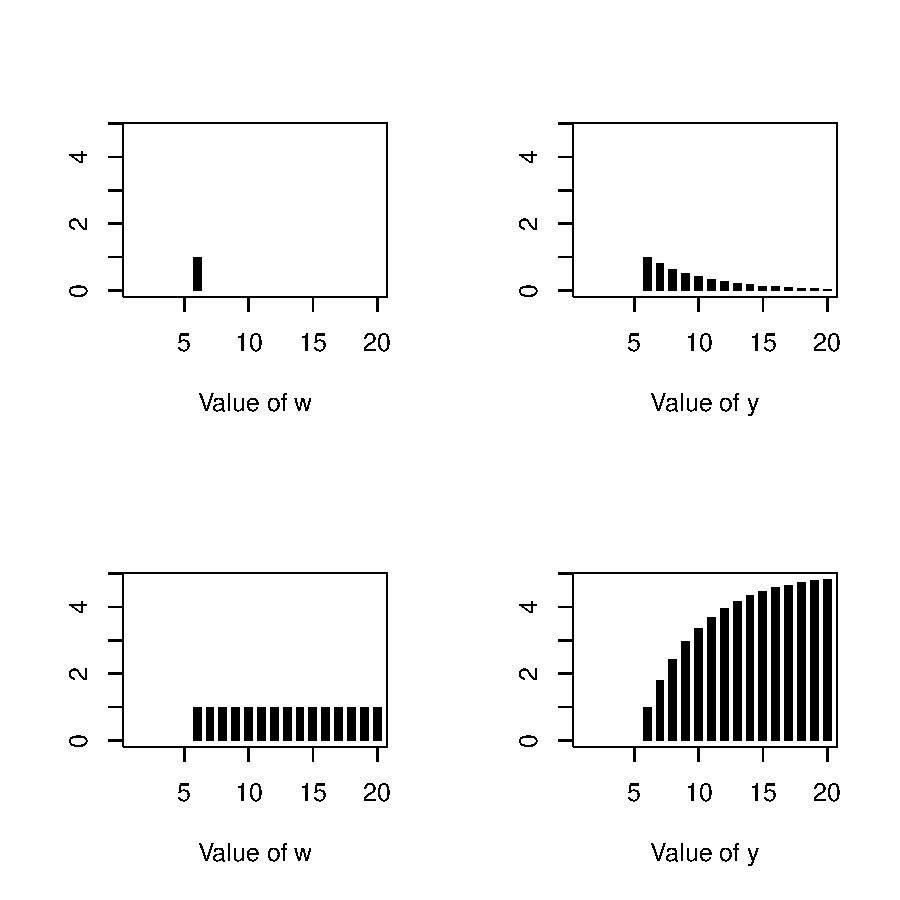
\includegraphics{Companion-010}
\end{center}
\subsection{Dynamic Multipliers for Second Order Difference Equations}
Finally we use similar techniques to calculate the effects of an impulse on a second order system.
Here each column of phi represents the coefficients of a second order system.
\begin{Schunk}
\begin{Sinput}
 T <- 20
 w <- 1 * (1:20 == 3)
 y <- array(dim = c(T, 2))
 y[1:2, ] <- 0
 phi <- array(c(0.6, 0.2, 0.5, -0.8), c(2, 2))
 for (j in 3:T) y[j, ] <- apply(X = phi * y[(j - 1):(j - 2), ], 
+     MARGIN = 2, FUN = sum) + w[j]
\end{Sinput}
\end{Schunk}
The results can be plotted reproducing figure 1.4.
\begin{center}
\includegraphics{Companion-012}
\end{center}
\section{Stationary ARMA Processes}
\subsection{Autocorrelations for AR and MA Processes}
Pages 50 to 59 describe the calculation of autocorrelation functions of AR and MA processes.
Following the expressions in the text we can calculate results using separate formulae for white
noise, moving average, and autoregressive processes.
\begin{Schunk}
\begin{Sinput}
 T <- 20
 specifications <- list(list(label = "White Noise", MA = vector(mode = "numeric"), 
+     AR = vector(mode = "numeric")), list(label = "MA(1)", MA = c(0.8), 
+     AR = vector(mode = "numeric")), list(label = "MA(4)", MA = c(-0.6, 
+     0.5, -0.5, 0.3), AR = vector(mode = "numeric")), list(label = "AR(1) with 0.8", 
+     MA = vector(mode = "numeric"), AR = c(0.8)), list(label = "AR(1) with -0.8", 
+     MA = vector(mode = "numeric"), AR = c(-0.8)))
 sigmasq <- 1
\end{Sinput}
\end{Schunk}
White noise calculations are described on bottom of page 47 and the top of page 48.
\begin{Schunk}
\begin{Sinput}
 specifications[[1]]$rho <- c(1, rep(0, T - 1))
\end{Sinput}
\end{Schunk}
Moving average calculations are described on page 51.
\begin{Schunk}
\begin{Sinput}
 for (i in 2:3) {
+     MA <- specifications[[i]]$MA
+     q <- length(MA)
+     gamma <- vector(mode = "numeric", length = T)
+     gamma[1] <- sigmasq * t(c(1, MA)) %*% c(1, MA)
+     for (j in 1:q) gamma[j + 1] <- sigmasq * t(MA[j:q]) %*% c(1, 
+         MA)[1:(q - j + 1)]
+     gamma[(q + 2):T] <- 0
+     specifications[[i]]$rho <- gamma/gamma[1]
+ }
\end{Sinput}
\end{Schunk}
Autocorrelation calculations are described on page 59
\begin{Schunk}
\begin{Sinput}
 for (i in 4:5) {
+     AR <- specifications[[i]]$AR
+     p <- length(AR)
+     F <- rbind(AR, cbind(diag(p - 1), rep(0, p - 1)))
+     gamma <- vector(mode = "numeric", length = T)
+     gamma[1:p] <- sigmasq * solve(diag(p^2) - F %x% F)[1:p, 1]
+     for (j in (p + 1):T) gamma[[j]] <- t(gamma[(j - 1):(j - p)]) %*% 
+         AR
+     specifications[[i]]$rho <- gamma/gamma[1]
+ }
\end{Sinput}
\end{Schunk}
\begin{center}
\includegraphics{Companion-017}
\end{center}
\subsection{R Facilities for ARMA Autocorrelations}
Function ARMAacf can be used to calculate autocorrelations for an arbitrary ARMA process.
\begin{Schunk}
\begin{Sinput}
 g3 <- ARMAacf(ar = numeric(0), ma = specifications[[3]]$MA, lag.max = T, 
+     pacf = FALSE)
 print(specifications[[3]]$rho)
\end{Sinput}
\begin{Soutput}
 [1]  1.0000000 -0.6666667  0.4871795 -0.3487179  0.1538462  0.0000000
 [7]  0.0000000  0.0000000  0.0000000  0.0000000  0.0000000  0.0000000
[13]  0.0000000  0.0000000  0.0000000  0.0000000  0.0000000  0.0000000
[19]  0.0000000  0.0000000
\end{Soutput}
\begin{Sinput}
 print(g3)
\end{Sinput}
\begin{Soutput}
         0          1          2          3          4          5          6 
 1.0000000 -0.6666667  0.4871795 -0.3487179  0.1538462  0.0000000  0.0000000 
         7          8          9         10         11         12         13 
 0.0000000  0.0000000  0.0000000  0.0000000  0.0000000  0.0000000  0.0000000 
        14         15         16         17         18         19         20 
 0.0000000  0.0000000  0.0000000  0.0000000  0.0000000  0.0000000  0.0000000 
\end{Soutput}
\begin{Sinput}
 g4 <- ARMAacf(ar = specifications[[4]]$AR, ma = numeric(0), lag.max = T - 
+     1, pacf = FALSE)
 print(specifications[[4]]$rho)
\end{Sinput}
\begin{Soutput}
 [1] 1.00000000 0.80000000 0.64000000 0.51200000 0.40960000 0.32768000
 [7] 0.26214400 0.20971520 0.16777216 0.13421773 0.10737418 0.08589935
[13] 0.06871948 0.05497558 0.04398047 0.03518437 0.02814750 0.02251800
[19] 0.01801440 0.01441152
\end{Soutput}
\begin{Sinput}
 print(g4)
\end{Sinput}
\begin{Soutput}
         0          1          2          3          4          5          6 
1.00000000 0.80000000 0.64000000 0.51200000 0.40960000 0.32768000 0.26214400 
         7          8          9         10         11         12         13 
0.20971520 0.16777216 0.13421773 0.10737418 0.08589935 0.06871948 0.05497558 
        14         15         16         17         18         19 
0.04398047 0.03518437 0.02814750 0.02251800 0.01801440 0.01441152 
\end{Soutput}
\end{Schunk}
\subsection{Autocorrelations as a Function of the Moving Average Parameter}
Figure 3.2 is easily generated from the formula for autocorrelations of an MA(1) process.
\begin{Schunk}
\begin{Sinput}
 theta <- (-300:300) * 0.01
 corrs <- theta/(1 + theta^2)
 plot(theta, corrs, type = "l")
 grid(nx = 2, ny = 2)
\end{Sinput}
\end{Schunk}
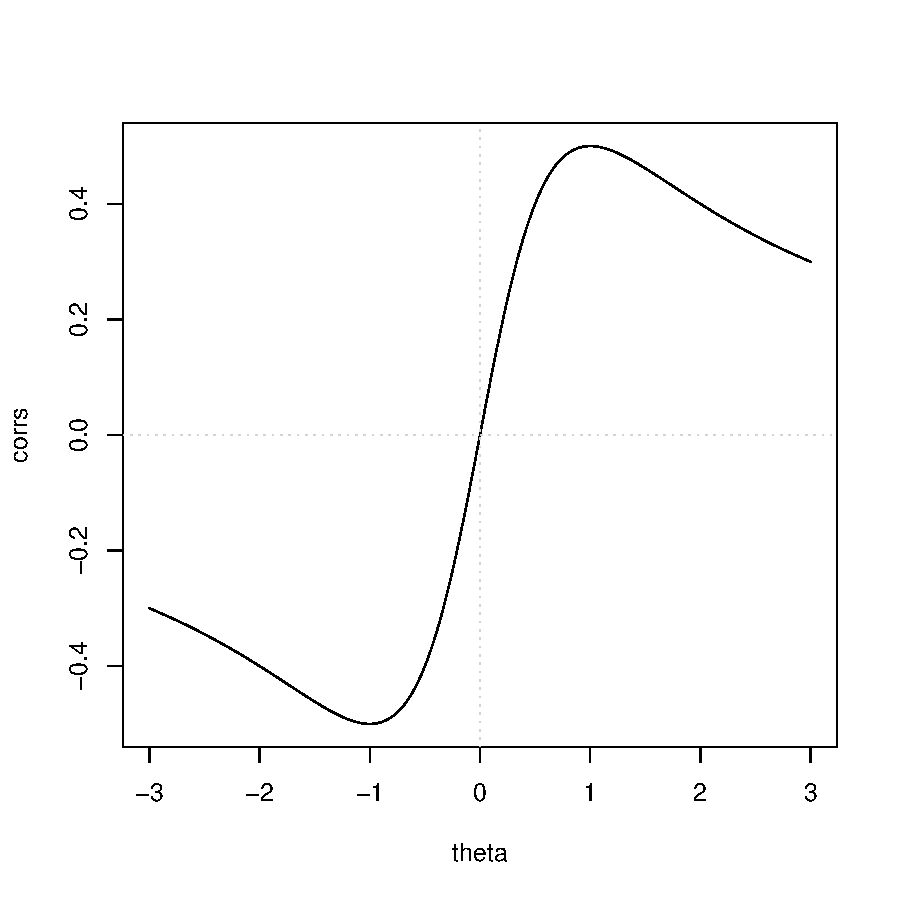
\includegraphics{Companion-019}
\subsection{Realizations of ARMA Processes}
Pages 55 shows some realizations of AR processes.  We will assume the innovations are
drawn from a standard normal distribution.
\begin{Schunk}
\begin{Sinput}
 specifications <- list(list(label = "f = 0", MA = vector(mode = "numeric"), 
+     AR = vector(mode = "numeric")), list(label = "f = .5", MA = vector(mode = "numeric"), 
+     AR = c(0.5)), list(label = "f = .9", MA = vector(mode = "numeric"), 
+     AR = c(0.9)))
 T <- 100
 epsilon <- rnorm(T, 0, 1)
\end{Sinput}
\end{Schunk}
These can be calculated by iterating forward on the defining equations.
\begin{Schunk}
\begin{Sinput}
 simulate.forward <- function(specification, epsilon) {
+     T <- length(epsilon)
+     AR <- specification$AR
+     MA <- specification$MA
+     presample <- rep(0, max(length(AR), length(MA)))
+     epsilon <- c(presample, epsilon)
+     Y <- vector(mode = "numeric", length = T + length(presample))
+     Y[1:length(presample)] <- 0
+     for (i in (length(presample) + 1):(T + length(presample))) Y[i] <- epsilon[[i]] + 
+         ifelse(length(AR) > 0, t(AR) %*% Y[(i - 1):(i - length(AR))], 
+             0) + ifelse(length(MA) > 0, t(MA) %*% epsilon[(i - 
+         1):(i - length(MA))], 0)
+     Y[(length(presample) + 1):(T + length(presample))]
+ }
 for (i in 1:length(specifications)) specifications[[i]]$Y <- simulate.forward(specifications[[i]], 
+     epsilon)
\end{Sinput}
\end{Schunk}
\begin{center}
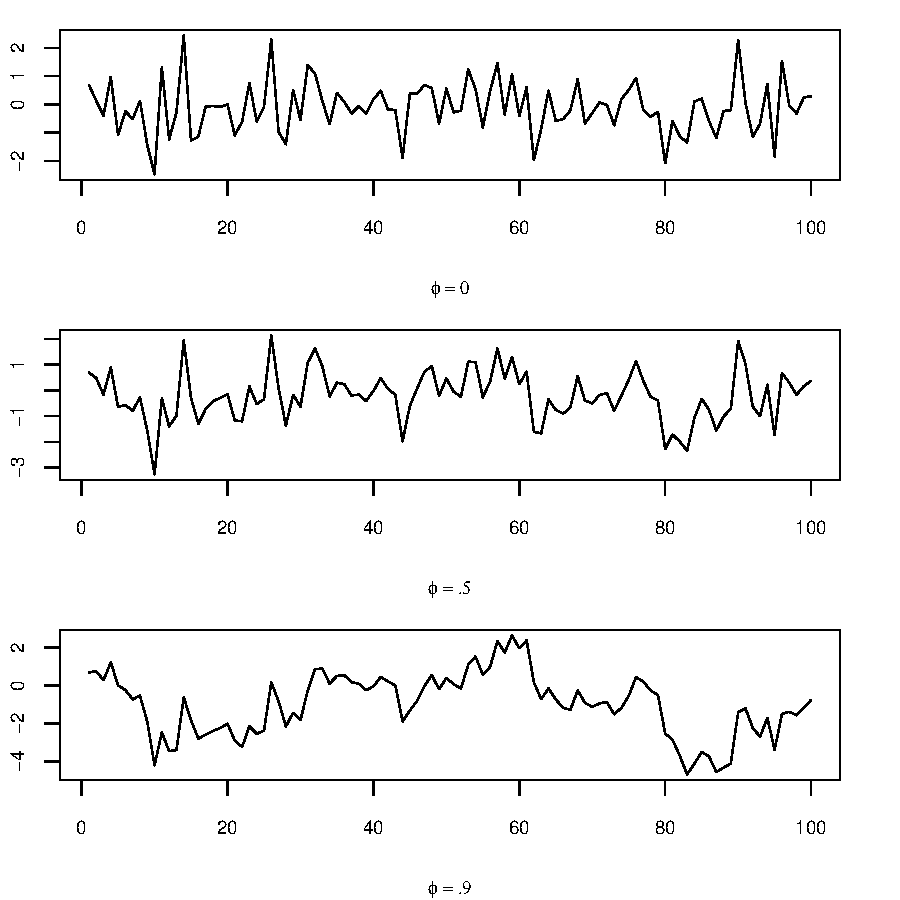
\includegraphics{Companion-022}
\end{center}
\subsection{R Facilities for simulating ARMA process}
Function "simulate.forward" is a special case of capabilities provided by
the function arima.sim in package stats, as the following code verifies.
\begin{Schunk}
\begin{Sinput}
 for (specification in specifications) {
+     AR <- specification$AR
+     MA <- specification$MA
+     shift <- max(length(AR), length(MA))
+     Y <- arima.sim(model = list(order = c(length(AR), 0, length(MA)), 
+         ar = AR, ma = MA), n = T, innov = epsilon[1:T], n.start = max(shift, 
+         1), start.innov = rep(0, max(shift, 1)))
+     print(specification$Y[1:10])
+     print(Y[1:10])
+ }
\end{Sinput}
\begin{Soutput}
 [1] -1.1980297 -1.4082553 -1.4978803 -1.4816348  0.1763239  0.3944134
 [7]  0.4618201 -1.2461269  0.0898164 -0.1254357
 [1] -1.1980297 -1.4082553 -1.4978803 -1.4816348  0.1763239  0.3944134
 [7]  0.4618201 -1.2461269  0.0898164 -0.1254357
 [1] -1.1980297 -2.0072701 -2.5015153 -2.7323925 -1.1898723 -0.2005227
 [7]  0.3615587 -1.0653476 -0.4428574 -0.3468644
 [1] -1.1980297 -2.0072701 -2.5015153 -2.7323925 -1.1898723 -0.2005227
 [7]  0.3615587 -1.0653476 -0.4428574 -0.3468644
 [1] -1.198030 -2.486482 -3.735714 -4.843777 -4.183076 -3.370355 -2.571499
 [8] -3.560476 -3.114612 -2.928587
 [1] -1.198030 -2.486482 -3.735714 -4.843777 -4.183076 -3.370355 -2.571499
 [8] -3.560476 -3.114612 -2.928587
\end{Soutput}
\end{Schunk}
\section{Sample Autocorrelations and Partial Autocorrelations}
\subsection{A Box Jenkins Example}
Example 4.1 from page 112 illustrates the Box-Jenkins
approach based on autocorrelations.  Here the data series is log changes
of seasonally adjusted real US GNP from 1947 to 1988,
available by simple transformations of the data in object "gnp1996".
The data is prepared by selecting quarterly date from as shown, then computing the log of differences.
\begin{Schunk}
\begin{Sinput}
 data(gnp1996, package = "Ham94")
 selection <- subset(gnp1996, Quarter >= "1947-01-01" & Quarter <= 
+     "1988-10-01")
 y <- diff(log(selection$GNPH))
\end{Sinput}
\end{Schunk}
Page 110 shows how to compute sample autocorrelations - we will generate the first 20 to be used in plotting the results below.
\begin{Schunk}
\begin{Sinput}
 max.lags <- 20
 T <- length(y)
 threshold <- 2/sqrt(T)
 gammas <- vector(mode = "numeric", length = max.lags + 1)
 gammas[[1]] <- 1/T * t(y - mean(y)) %*% (y - mean(y))
 for (j in 1:max.lags) gammas[j + 1] <- 1/T * t((y - mean(y))[(j + 
+     1):T]) %*% (y - mean(y))[1:(T - j)]
 rhos <- gammas/gammas[[1]]
\end{Sinput}
\end{Schunk}
Page 111 shows how to compute sample partial autocorrelations.  
\begin{Schunk}
\begin{Sinput}
 subscripts <- outer(seq(1, max.lags), seq(1, max.lags), function(i, 
+     j) {
+     abs(i - j)
+ })
 GAMMA <- array(gammas[as.vector(subscripts) + 1], c(max.lags, 
+     max.lags))
 alphas <- vector(mode = "numeric", length = max.lags)
 for (m in 1:max.lags) alphas[m] <- solve(GAMMA[1:m, 1:m], gammas[2:(m + 
+     1)])[[m]]
\end{Sinput}
\end{Schunk}
A plot of the outputs reproducing figure 4.2 is shown below.  The source code is provided in the demo.
\begin{center}
\includegraphics{Companion-027}
\end{center}
\subsection{R Facilities for Sample Autocorrelations}
Function acf from R package "stats" performs the same function as acf, as we can readily
confirm.
\begin{Schunk}
\begin{Sinput}
 acf.correlation <- acf(y, lag.max = max.lags, type = "correlation", 
+     plot = FALSE, demean = TRUE)
 print(as.vector(acf.correlation$acf))
\end{Sinput}
\begin{Soutput}
 [1]  1.00000000  0.34509475  0.17817758 -0.02537843 -0.14230681 -0.18827409
 [7] -0.11613672 -0.09335581 -0.04441490  0.03902657  0.05412612  0.03788102
[13] -0.12386994 -0.12725888 -0.10256196 -0.10719806  0.05022865  0.07874423
[19]  0.10451845  0.05540046  0.07001701
\end{Soutput}
\begin{Sinput}
 print(rhos)
\end{Sinput}
\begin{Soutput}
 [1]  1.00000000  0.34509475  0.17817758 -0.02537843 -0.14230681 -0.18827409
 [7] -0.11613672 -0.09335581 -0.04441490  0.03902657  0.05412612  0.03788102
[13] -0.12386994 -0.12725888 -0.10256196 -0.10719806  0.05022865  0.07874423
[19]  0.10451845  0.05540046  0.07001701
\end{Soutput}
\begin{Sinput}
 acf.partial <- acf(y, lag.max = max.lags, type = "partial", plot = FALSE, 
+     demean = TRUE)
 print(as.vector(acf.partial$acf))
\end{Sinput}
\begin{Soutput}
 [1]  0.345094750  0.067075208 -0.120748043 -0.128609341 -0.096659383
 [6]  0.006935269 -0.040052970 -0.027544630  0.043507786  0.007543470
[11] -0.020592065 -0.186352407 -0.053599417  0.009939122 -0.066137883
[16]  0.093638650  0.007111983  0.016895000 -0.045185857  0.023227306
\end{Soutput}
\begin{Sinput}
 print(alphas)
\end{Sinput}
\begin{Soutput}
 [1]  0.345094750  0.067075208 -0.120748043 -0.128609341 -0.096659383
 [6]  0.006935269 -0.040052970 -0.027544630  0.043507786  0.007543470
[11] -0.020592065 -0.186352407 -0.053599417  0.009939122 -0.066137883
[16]  0.093638650  0.007111983  0.016895000 -0.045185857  0.023227306
\end{Soutput}
\end{Schunk}

\section{Spectral Analysis}
Pages 167 to 170 give an example of the uses of spectral analysis, as applied to US Industrial Production from
January 1947 to November 1989, available in data source "indprod".  We will analyze the actual raw data, as well as
one month and one year log changes.
\begin{Schunk}
\begin{Sinput}
 data(indprod, package = "Ham94")
 selection <- subset(indprod, Month >= "1947-01-01" & Month <= 
+     "1989-11-01")
 raw.data <- selection$IPMFG6
 logdiff.data <- 100 * diff(log(raw.data), lag = 1)
 yeardiff.data <- 100 * diff(log(raw.data), lag = 12)
\end{Sinput}
\end{Schunk}
For plotting purposes, generate frequencies at regular intervals as show on page 159.  The first
spectrum uses unsmoothed estimates, the last two use a Bartlett kernel.

We show this in two ways:	
\begin{itemize}
\item Step by step function (page \pageref{par:Chap6Man})
\item Built-in function (page \pageref{par:Chap6Auto})
\end{itemize}
\paragraph{Step by step function\label{par:Chap6Man}}
\begin{Schunk}
\begin{Sinput}
 s.Y.omega <- function(omega, gammas, params) {
+     1/(2 * pi) * (gammas[[1]] + 2 * as.numeric(t(gammas[-1]) %*% 
+         cos(1:(length(gammas) - 1) * omega)))
+ }
 s.Y.omega.Bartlett <- function(omega, gammas, params) {
+     1/(2 * pi) * (gammas[[1]] + 2 * as.numeric(t((1 - 1:params/(params + 
+         1)) * gammas[2:(params + 1)]) %*% cos(1:params * omega)))
+ }
 generate.plot.data <- function(values, estimator, params) {
+     T <- length(values)
+     acf.covariance <- acf(values, lag.max = T - 1, type = "covariance", 
+         plot = FALSE, demean = TRUE)
+     sapply(2 * pi/T * 1:((T - 1)/2), estimator, as.vector(acf.covariance$acf), 
+         params)
+ }
 raw.s.Y.omega <- generate.plot.data(raw.data, s.Y.omega, NULL)
 logdiff.s.Y.omega <- generate.plot.data(logdiff.data, s.Y.omega.Bartlett, 
+     12)
 yeardiff.s.Y.omega <- generate.plot.data(yeardiff.data, s.Y.omega.Bartlett, 
+     12)
\end{Sinput}
\end{Schunk}
The resulting output is shown below.
\begin{center}
\includegraphics{Companion-031}

\paragraph{Built-in function\label{par:Chap6Auto}}
We use here the function spectrum:

\begin{Schunk}
\begin{Sinput}
 args(spectrum)
\end{Sinput}
\begin{Soutput}
function (x, ..., method = c("pgram", "ar")) 
NULL
\end{Soutput}
\end{Schunk}
\begin{Schunk}
\begin{Sinput}
 sp <- spectrum(raw.data, plot = FALSE, span = 10)
 x <- 100 * diff(log(raw.data))
 sp2 <- spectrum(x, span = 6, plot = FALSE)
 x12 <- 100 * diff(log(raw.data), lag = 12)
 sp3 <- spectrum(x12, span = 20, plot = FALSE)
\end{Sinput}
\end{Schunk}
The resulting output is shown below.
\includegraphics{Companion-034}
\end{center}

\section{The Kalman Filter}
\subsection{Kalman Filtering Example Applied to Detecting Business Cycles}
Page 376 describes an application of Kalman filtering to business cycles by James Stock and Mark Watson.

This can be implemented in two steps.  The first is to implement the Kalman algorithm as described in the text.  The
following function follows the notation in Chapter 13.
\begin{Schunk}
\begin{Sinput}
 kalman <- function(H, R, F, x, A, y, Q, xi.1.0, P.1.0) {
+     T <- dim(x)[[2]]
+     P.t.t_1 <- array(dim = c(dim(P.1.0), T + 1))
+     P.t.t_1[, , 1] <- P.1.0
+     P.t.t <- array(dim = c(dim(P.1.0), T))
+     K.t <- array(dim = c(dim(H), T))
+     xi.t.t_1 <- array(dim = c(length(xi.1.0), T + 1))
+     xi.t.t_1[, 1] <- xi.1.0
+     xi.t.t <- array(dim = c(length(xi.1.0), T))
+     L <- 0
+     for (tt in 1:T) {
+         V <- solve(t(H) %*% P.t.t_1[, , tt] %*% H + R)
+         K.t[, , tt] <- P.t.t_1[, , tt] %*% H %*% V
+         P.t.t[, , tt] <- P.t.t_1[, , tt] - K.t[, , tt] %*% t(H) %*% 
+             P.t.t_1[, , tt]
+         P.t.t_1[, , tt + 1] <- F %*% P.t.t[, , tt] %*% t(F) + 
+             Q
+         w <- y[, tt] - t(A) %*% x[, tt] - t(H) %*% xi.t.t_1[, 
+             tt]
+         xi.t.t[, tt] <- xi.t.t_1[, tt] + K.t[, , tt] %*% w
+         xi.t.t_1[, tt + 1] <- F %*% xi.t.t[, tt]
+         L <- L - 1/2 * dim(y)[[1]] * log(2 * pi) + 1/2 * log(det(V)) - 
+             1/2 * t(w) %*% V %*% w
+     }
+     xi.t.T <- array(dim = c(length(xi.1.0), T))
+     xi.t.T[, T] <- xi.t.t[, T]
+     P.t.T <- array(dim = c(dim(P.1.0), T))
+     P.t.T[, , T] <- P.t.t[, , T]
+     for (tt in (T - 1):1) {
+         Jt <- P.t.t[, , tt] %*% t(F) %*% solve(P.t.t_1[, , tt + 
+             1])
+         xi.t.T[, tt] <- xi.t.t[, tt] + Jt %*% (xi.t.T[, tt + 
+             1] - xi.t.t_1[, tt + 1])
+         P.t.T[, , tt] <- P.t.t[, , tt] + Jt %*% (P.t.T[, , tt + 
+             1] - P.t.t_1[, , tt + 1]) %*% t(Jt)
+     }
+     list(xi.t.t = xi.t.t, xi.t.t_1 = xi.t.t_1, P.t.t = P.t.t, 
+         P.t.t_1 = P.t.t_1, K.t = K.t, log.likelihood = L, xi.t.T = xi.t.T, 
+         P.t.T = P.t.T)
+ }
\end{Sinput}
\end{Schunk}
The second is to specify the state space model as described on pp376-377 and estimate the parameters
via maximum likelihood.  Data for this analysis is consumption and income data form dataset "coninc" in log differences.
\begin{Schunk}
\begin{Sinput}
 data(coninc, package = "Ham94")
 YGR <- diff(log(coninc$GYD82))
 CGR <- diff(log(coninc$GC82))
 y <- t(cbind(YGR - mean(YGR), CGR - mean(CGR)))
\end{Sinput}
\end{Schunk}
The following helper function converts the parameters from a vector of labeled
components into the correct inputs for the filter as shown in equations [13.1.28], [13.1.29], and [13.1.30].
\begin{Schunk}
\begin{Sinput}
 THETA <- c(phic = 0.9, phi1 = 0.9, phi2 = 0.9, g1 = 0.5, g2 = 0.5, 
+     sigc = 0.05^0.5, sig11 = 0.05^0.5, sig22 = 0.05^0.5, r11 = sd(YGR), 
+     r22 = sd(CGR))
 theta.y.to.params <- function(THETA, y) {
+     params <- list(F = diag(THETA[c("phic", "phi1", "phi2")]), 
+         Q = diag(THETA[c("sigc", "sig11", "sig22")]^2), H = rbind(THETA[c("g1", 
+             "g2")], diag(2)), R = diag(THETA[c("r11", "r22")]^2), 
+         A = diag(c(0, 0)), x = c(1, 1) %o% rep(1, dim(y)[[2]]), 
+         xi.1.0 = c(0, 0, 0))
+     c(params, list(P.1.0 = array(solve(diag(length(params$xi.1.0)^2) - 
+         params$F %x% params$F, as.vector(params$Q)), c(length(params$xi.1.0), 
+         length(params$xi.1.0)))))
+ }
\end{Sinput}
\end{Schunk}
The objective function is the log.likelihood obtained from the Kalman iteration.
\begin{Schunk}
\begin{Sinput}
 objective <- function(THETA, y) {
+     params <- theta.y.to.params(THETA, y)
+     kalman(params$H, params$R, params$F, params$x, params$A, 
+         y, params$Q, params$xi.1.0, params$P.1.0)$log.likelihood
+ }
 optimizer.results <- optim(par = THETA, fn = objective, gr = NULL, 
+     y = y, control = list(trace = 0))
\end{Sinput}
\end{Schunk}
Finally calculate the smoothed results based on the ML estimated parameters.
\begin{Schunk}
\begin{Sinput}
 params <- theta.y.to.params(optimizer.results$par, y)
 smoothed.results <- kalman(params$H, params$R, params$F, params$x, 
+     params$A, y, params$Q, params$xi.1.0, params$P.1.0)
 smoothed.data <- smoothed.results$xi.t.T[1, ]
\end{Sinput}
\end{Schunk}
The results of the smoothed inference are shown below.
\begin{center}
\includegraphics{Companion-040}
\end{center}
\subsection{R facilities for Kalman Filtering}
There are several different packages in R for Kalman filtering, some that provide univariate support,
others multivariate support.  For example, package FKF is a fast implementation, but there are others. One key
aspect of using such packages is specifying an interface to allow for time varying inputs, and providing results
under those conditions.  Some packages use caller supplied functions, others check for dimensions of (up to three
dimensional) arrays, etc.

For example, a simple implementation of the example on page 382 using function "kalman" above might look like:
\begin{Schunk}
\begin{Sinput}
 sigmasq <- 2
 params <- list(F = array(c(0, 1, 0, 0), c(2, 2)), Q = diag(c(sigmasq, 
+     0)), H = array(c(1, 0.8), c(2, 1)), R = array(0, c(1, 1)), 
+     A = array(0.5, c(1, 1)), x = 1 %o% rep(1, 5), y = 1 %o% c(1, 
+         seq(0.5, 4)), xi.1.0 = c(0, 0))
 params <- c(params, list(P.1.0 = array(solve(diag(length(params$xi.1.0)^2) - 
+     params$F %x% params$F, as.vector(params$Q)), c(length(params$xi.1.0), 
+     length(params$xi.1.0)))))
 myResults <- kalman(params$H, params$R, params$F, params$x, params$A, 
+     params$y, params$Q, params$xi.1.0, params$P.1.0)
\end{Sinput}
\end{Schunk}
We can perform the some operations using package FKF with a slight alteration of the function arguments.
In particular, many of the arguments using an outer product as a quick way to convert them into a structure
of one additional dimension, with the length of the additional dimension being 1.  This is a convenient calling convention to specifying a *non* time varying parameter.  If the
parameter *were* time varying then the full extra dimension would be used.
For example, the F matrix can
be time varying in FKF (called Tt).  A call exploiting this would then have a vector of two dimensional F matrices, one
for each time index, i.e. a three dimensional array.  If F is not time varying, (as in the case of the simple
example above) then a three dimensional array with the
third dimension being of length 1 is used.
\begin{Schunk}
\begin{Sinput}
 fkfResults <- FKF::fkf(a0 = params$xi.1.0, P0 = params$P.1.0, 
+     dt = rep(0, length(params$xi.1.0)) %o% 1, Tt = params$F %o% 
+         1, HHt = params$Q %o% 1, ct = t(params$A) %*% params$x, 
+     Zt = t(params$H) %o% 1, GGt = params$R %o% 1, yt = params$y, 
+     check.input = TRUE)
\end{Sinput}
\end{Schunk}
The results can be confirmed by examing the output:
\begin{Schunk}
\begin{Sinput}
 print(myResults$xi.t.t)
\end{Sinput}
\begin{Soutput}
          [,1]       [,2]        [,3]     [,4]     [,5]
[1,] 0.3048780 -0.1951600  1.02502699 1.100137 2.031900
[2,] 0.2439024  0.2439500 -0.03128374 1.124828 1.210125
\end{Soutput}
\begin{Sinput}
 print(fkfResults$att)
\end{Sinput}
\begin{Soutput}
          [,1]       [,2]        [,3]     [,4]     [,5]
[1,] 0.3048780 -0.1951600  1.02502699 1.100137 2.031900
[2,] 0.2439024  0.2439500 -0.03128374 1.124828 1.210125
\end{Soutput}
\end{Schunk}

\section{Generalized Method of Moments}
\subsection{Classical Method of Moments}
Pages 409-410 gives a simple example of estimating the degrees of freedom of a standard t distribution. 
To illustrate, first generate a sample of 500 observations from a t distribution with 10 degrees of freedom.
\begin{Schunk}
\begin{Sinput}
 Y <- rt(500, 10)
\end{Sinput}
\end{Schunk}
Then maximize the sum of logs of a t density evaluated on the sample points.
\begin{Schunk}
\begin{Sinput}
 objective <- function(nu, Y) {
+     -sum(log(dt(Y, df = nu)))
+ }
 classical.results <- optimize(interval = c(1, 30), f = objective, 
+     Y = Y)
 mu2 <- mean(Y^2)
 nu <- 2 * mu2/(mu2 - 1)
 print(classical.results)
\end{Sinput}
\begin{Soutput}
$minimum
[1] 10.04124

$objective
[1] 748.1768
\end{Soutput}
\begin{Sinput}
 print(nu)
\end{Sinput}
\begin{Soutput}
[1] 12.27138
\end{Soutput}
\end{Schunk}
\subsection{Generalized Method of Moments}
Using the sample sample, we can estimate the degrees of freedom using GMM.  To this end define a
function following the GMM recipe in the text.  
\begin{Schunk}
\begin{Sinput}
 compute.estimates <- function(Y, h, interval) {
+     g <- function(Y, THETA) {
+         apply(X = apply(X = Y, MARGIN = 1, FUN = h, THETA = THETA), 
+             MARGIN = 1, FUN = mean)
+     }
+     objective <- function(THETA, Y, W) {
+         g.value <- g(Y, THETA)
+         t(g.value) %*% W %*% g.value
+     }
+     r <- length(h(Y[1, ], interval[[1]]))
+     a <- length(interval[[1]])
+     T <- dim(Y)[[1]]
+     stage.1.results <- optimize(interval = interval, f = objective, 
+         Y = Y, W = diag(r))
+     temp <- apply(X = Y, MARGIN = 1, FUN = h, THETA = stage.1.results$objective)
+     S <- 1/T * temp %*% t(temp)
+     stage.2.results <- optimize(interval = interval, f = objective, 
+         Y = Y, W = solve(S))
+     J.test <- 1 - pchisq(T * stage.2.results$objective, r - a)
+     list(stage.1.results = stage.1.results, stage.2.results = stage.2.results, 
+         overidentifying = J.test)
+ }
\end{Sinput}
\end{Schunk}
Using this function is then a matter of specifying an appropriate function h to define an observation of
the set of moments being targeted.
\begin{Schunk}
\begin{Sinput}
 h <- function(Yt, THETA) {
+     nu <- THETA
+     c(Yt^2 - nu/(nu - 2), Yt^4 - 3 * nu^2/((nu - 2) * (nu - 4)))
+ }
 estimates <- compute.estimates(Y %o% 1, h, interval = c(5, 30))
 print(estimates)
\end{Sinput}
\begin{Soutput}
$stage.1.results
$stage.1.results$minimum
[1] 11.53954

$stage.1.results$objective
             [,1]
[1,] 0.0002239881


$stage.2.results
$stage.2.results$minimum
[1] 11.15862

$stage.2.results$objective
             [,1]
[1,] 0.0001238368


$overidentifying
          [,1]
[1,] 0.8034891
\end{Soutput}
\end{Schunk}
A second example estimates the shape parameter of a two-sided gamma distribution.
\begin{Schunk}
\begin{Sinput}
 Yg <- rgamma(500, 10) * sign(runif(500, -1, 1))
 hg <- function(Yt, THETA) {
+     k <- THETA
+     nu <- k
+     mu <- k
+     sigma <- k
+     skew <- 2/sqrt(k)
+     kurt <- 6/k
+     c(Yt^2 - sigma - mu^2, Yt^4 - (kurt * (sigma^2) + 3) - 4 * 
+         (skew * sigma^1.5) * mu - 6 * sigma * mu^2 - mu^4)
+ }
 gestimates <- compute.estimates(Yg %o% 1, hg, interval = c(5, 
+     30))
 print(gestimates)
\end{Sinput}
\begin{Soutput}
$stage.1.results
$stage.1.results$minimum
[1] 9.8264

$stage.1.results$objective
         [,1]
[1,] 2.987595


$stage.2.results
$stage.2.results$minimum
[1] 9.789797

$stage.2.results$objective
            [,1]
[1,] 0.000909186


$overidentifying
          [,1]
[1,] 0.5001618
\end{Soutput}
\end{Schunk}
\subsection{R Facilities for Generalized Method of Moments}
TBD
\section{Models of Nonstationary Time Series}
\subsection{Fractional Integration}
This example uses package fracdiff to compute the exponent of fractional integration as described on pp448-449.
Data is US GDP and Treasury Yields.
\begin{Schunk}
\begin{Sinput}
 data(gnptbill, package = "Ham94")
 print(fdGPH(gnptbill$GNP))
\end{Sinput}
\begin{Soutput}
$d
[1] 0.9588756

$sd.as
[1] 0.2427173

$sd.reg
[1] 0.04061276
\end{Soutput}
\begin{Sinput}
 print(fdGPH(gnptbill$TBILL))
\end{Sinput}
\begin{Soutput}
$d
[1] 0.9511594

$sd.as
[1] 0.2427173

$sd.reg
[1] 0.227921
\end{Soutput}
\end{Schunk}
\section{Univariate Processes with Unit Roots}
\subsection{Preamble}
This section uses a few utility functions that follow procedures in the test for testing hypotheses about unit roots.
First is the Newey West estimator described by [10.5.10] and [10.5.15].
\begin{Schunk}
\begin{Sinput}
 print(Newey.West)
\end{Sinput}
\begin{Soutput}
function (X, lags) 
{
    S <- 0
    T <- dim(X)[[1]]
    for (lag in lags:1) S <- S + (lags + 1 - lag)/(lags + 1) * 
        t(X[(lag + 1):T, ]) %*% X[1:(T - lag), ]
    1/T * (t(X) %*% X + S + t(S))
}
<environment: namespace:Ham94>
\end{Soutput}
\end{Schunk}
Next are the Dickey Fuller stats described in [17.4.7] and [17.4.9], with an optional correction for
serial correlation defined in [17.7.35] and [17.7.38].
\begin{Schunk}
\begin{Sinput}
 print(Dickey.Fuller)
\end{Sinput}
\begin{Soutput}
function (T, rho, sigma.rho, zeta = numeric(0)) 
{
    list(T = T, rho = rho, sigma.rho = sigma.rho, zeta = zeta, 
        rho.stat = T * (rho - 1)/(1 - sum(zeta)), t.stat = (rho - 
            1)/sigma.rho)
}
<environment: namespace:Ham94>
\end{Soutput}
\end{Schunk}
The Phillips Perron stats are defined by [17.6.8] and [17.6.12]
\begin{Schunk}
\begin{Sinput}
 print(Phillips.Perron)
\end{Sinput}
\begin{Soutput}
function (T, rho, sigma.rho, s, lambda.hat.sq, gamma0) 
{
    list(T = T, rho = rho, sigma.rho = sigma.rho, s.sq = s^2, 
        lambda.hat.sq = lambda.hat.sq, gamma0 = gamma0, rho.stat = T * 
            (rho - 1) - 1/2 * (T * sigma.rho/s)^2 * (lambda.hat.sq - 
            gamma0), t.stat = (gamma0/lambda.hat.sq)^0.5 * (rho - 
            1)/sigma.rho - 1/2 * (lambda.hat.sq - gamma0) * T * 
            sigma.rho/s/(lambda.hat.sq^0.5))
}
<environment: namespace:Ham94>
\end{Soutput}
\end{Schunk}
Finally the Wald form of an F test as defined by [8.1.32].
\begin{Schunk}
\begin{Sinput}
 print(Wald.F.Test)
\end{Sinput}
\begin{Soutput}
function (R, b, r, s2, XtX_1) 
{
    v <- R %*% b - r
    as.numeric(t(v) %*% solve(s2 * R %*% XtX_1 %*% t(R)) %*% 
        v/dim(R)[[1]])
}
<environment: namespace:Ham94>
\end{Soutput}
\end{Schunk}
\subsection{Dickey Fuller Tests for Unit Roots}
Page 489 describes the analysis of nominal
three month U.S. Treasury
yield data from
dataset gnptbill, shown below.
\begin{Schunk}
\begin{Sinput}
 data(gnptbill, package = "Ham94")
 tbill.data <- data.frame(yt = gnptbill$TBILL[-1], yt_1 = gnptbill$TBILL[-length(gnptbill$TBILL)])
\end{Sinput}
\end{Schunk}
\begin{center}
\includegraphics{Companion-055}
\end{center}
The regression model is shown in [17.4.13], and the results are shown below.
\begin{Schunk}
\begin{Sinput}
 case1.lms <- summary(lm(yt ~ 0 + yt_1 + 0, tbill.data))
 case1.DF <- Dickey.Fuller(T = length(tbill.data$yt), rho = case1.lms$coefficients[["yt_1", 
+     "Estimate"]], sigma.rho = case1.lms$coefficients[["yt_1", 
+     "Std. Error"]])
 print(case1.lms$coefficients)
\end{Sinput}
\begin{Soutput}
      Estimate Std. Error  t value      Pr(>|t|)
yt_1 0.9969357 0.01059183 94.12311 1.277207e-146
\end{Soutput}
\begin{Sinput}
 print(case1.DF)
\end{Sinput}
\begin{Soutput}
$T
[1] 168

$rho
[1] 0.9969357

$sigma.rho
[1] 0.01059183

$zeta
numeric(0)

$rho.stat
[1] -0.5147943

$t.stat
[1] -0.2893034
\end{Soutput}
\end{Schunk}
A similar analysis is described on page 494 , but a constant is included in the regression model [17.4.37].
\begin{Schunk}
\begin{Sinput}
 case2.lms <- summary(lm(yt ~ 1 + yt_1, tbill.data))
 case2.DF <- Dickey.Fuller(T = length(tbill.data$yt), rho = case2.lms$coefficients[["yt_1", 
+     "Estimate"]], sigma.rho = case2.lms$coefficients[["yt_1", 
+     "Std. Error"]])
 print(case2.lms$coefficients)
\end{Sinput}
\begin{Soutput}
             Estimate Std. Error   t value      Pr(>|t|)
(Intercept) 0.2105899 0.11212302  1.878204  6.210685e-02
yt_1        0.9669104 0.01913305 50.536135 1.013453e-102
\end{Soutput}
\begin{Sinput}
 print(case2.DF)
\end{Sinput}
\begin{Soutput}
$T
[1] 168

$rho
[1] 0.9669104

$sigma.rho
[1] 0.01913305

$zeta
numeric(0)

$rho.stat
[1] -5.559061

$t.stat
[1] -1.729450
\end{Soutput}
\end{Schunk}
Example 17.5 describes how to test the joint hypothesis that the trend coefficient is 0 and the autoregressive
coefficient is 1.
\begin{Schunk}
\begin{Sinput}
 F <- Wald.F.Test(R = diag(2), b = case2.lms$coefficients[, "Estimate"], 
+     r = c(0, 1), s2 = case2.lms$sigma^2, XtX_1 = case2.lms$cov.unscaled)
 print(F)
\end{Sinput}
\begin{Soutput}
[1] 1.806307
\end{Soutput}
\end{Schunk}
\subsection{Analyzing GNP data}
A similar analysis can be conducted on log real GNP data described beginning on page 501, shown below.
\begin{Schunk}
\begin{Sinput}
 logGNP <- 100 * log(gnptbill$GNP)
 gnp.data <- data.frame(tt = seq(1, length(gnptbill$GNP) - 1), 
+     yt = logGNP[-1], yt_1 = logGNP[-length(gnptbill$GNP)])
\end{Sinput}
\end{Schunk}
\includegraphics{Companion-060}
The regression model here incorporates a time trend, based on the shape of the GDP graph
\begin{Schunk}
\begin{Sinput}
 case4.lms <- summary(lm(yt ~ 1 + yt_1 + tt, gnp.data))
 case4.DF <- Dickey.Fuller(T = length(gnp.data$yt), rho = case4.lms$coefficients[["yt_1", 
+     "Estimate"]], sigma.rho = case4.lms$coefficients[["yt_1", 
+     "Std. Error"]])
 print(case4.lms$coefficients)
\end{Sinput}
\begin{Soutput}
               Estimate  Std. Error   t value      Pr(>|t|)
(Intercept) 27.26477184 13.54992552  2.012171  4.582876e-02
yt_1         0.96252203  0.01930452 49.859941 2.076152e-101
tt           0.02753238  0.01520877  1.810296  7.206931e-02
\end{Soutput}
\begin{Sinput}
 print(case4.DF)
\end{Sinput}
\begin{Soutput}
$T
[1] 168

$rho
[1] 0.962522

$sigma.rho
[1] 0.01930452

$zeta
numeric(0)

$rho.stat
[1] -6.296298

$t.stat
[1] -1.941409
\end{Soutput}
\begin{Sinput}
 F <- Wald.F.Test(R = cbind(rep(0, 2), diag(2)), b = case4.lms$coefficients[, 
+     "Estimate"], r = c(1, 0), s2 = case4.lms$sigma^2, XtX_1 = case4.lms$cov.unscaled)
 print(F)
\end{Sinput}
\begin{Soutput}
[1] 2.442251
\end{Soutput}
\end{Schunk}

\subsection{Using Phillips Perron Tests}
Examples 17.6 and 17.7 reanalyze the case 2 and case 4 regressions above using the Phillips Perron tests
as shown on pages 511-513.
\begin{Schunk}
\begin{Sinput}
 case2.PP <- Phillips.Perron(T = length(case2.lms$residuals), 
+     rho = case2.lms$coefficients[["yt_1", "Estimate"]], sigma.rho = case2.lms$coefficients[["yt_1", 
+         "Std. Error"]], s = case2.lms$sigma, lambda.hat.sq = as.numeric(Newey.West(case2.lms$residuals %o% 
+         1, 4)), gamma0 = mean(case2.lms$residuals^2))
 print(case2.lms$coefficients)
\end{Sinput}
\begin{Soutput}
             Estimate Std. Error   t value      Pr(>|t|)
(Intercept) 0.2105899 0.11212302  1.878204  6.210685e-02
yt_1        0.9669104 0.01913305 50.536135 1.013453e-102
\end{Soutput}
\begin{Sinput}
 print(case2.PP)
\end{Sinput}
\begin{Soutput}
$T
[1] 168

$rho
[1] 0.9669104

$sigma.rho
[1] 0.01913305

$s.sq
[1] 0.6375998

$lambda.hat.sq
[1] 0.6880069

$gamma0
[1] 0.6300093

$rho.stat
[1] -6.028975

$t.stat
[1] -1.795686
\end{Soutput}
\begin{Sinput}
 case4.PP <- Phillips.Perron(T = length(case4.lms$residuals), 
+     rho = case4.lms$coefficients[["yt_1", "Estimate"]], sigma.rho = case4.lms$coefficients[["yt_1", 
+         "Std. Error"]], s = case4.lms$sigma, lambda.hat.sq = as.numeric(Newey.West(case4.lms$residuals %o% 
+         1, 4)), gamma0 = mean(case4.lms$residuals^2))
 print(case4.lms$coefficients)
\end{Sinput}
\begin{Soutput}
               Estimate  Std. Error   t value      Pr(>|t|)
(Intercept) 27.26477184 13.54992552  2.012171  4.582876e-02
yt_1         0.96252203  0.01930452 49.859941 2.076152e-101
tt           0.02753238  0.01520877  1.810296  7.206931e-02
\end{Soutput}
\begin{Sinput}
 print(case4.PP)
\end{Sinput}
\begin{Soutput}
$T
[1] 168

$rho
[1] 0.962522

$sigma.rho
[1] 0.01930452

$s.sq
[1] 1.156270

$lambda.hat.sq
[1] 2.117173

$gamma0
[1] 1.135623

$rho.stat
[1] -10.76066

$t.stat
[1] -2.439143
\end{Soutput}
\end{Schunk}
\subsection{Augmented Dickey Fuller Tests}
Example 17.8 illustrates incorporates the use of lagged regressors to (putatively) eliminate serial
correlation in the residuals.  The function "embed" is useful for creating lagged regressors.
\begin{Schunk}
\begin{Sinput}
 tbill.data <- list(it = gnptbill$TBILL[-1:-5], delta.it_ = embed(diff(gnptbill$TBILL[-length(gnptbill$TBILL)]), 
+     4), it_1 = gnptbill$TBILL[c(-1:-4, -(length(gnptbill$TBILL):length(gnptbill$TBILL)))])
 tbill.lms <- summary(lm(it ~ delta.it_ + 1 + it_1, tbill.data))
 tbill.adf <- Dickey.Fuller(T = length(gnptbill$TBILL) - 5, rho = tbill.lms$coefficients[["it_1", 
+     "Estimate"]], sigma.rho = tbill.lms$coefficients[["it_1", 
+     "Std. Error"]], zeta = tbill.lms$coefficients[paste("delta.it", 
+     1:4, sep = "_"), "Estimate"])
 print(tbill.lms$coefficients)
\end{Sinput}
\begin{Soutput}
              Estimate Std. Error   t value      Pr(>|t|)
(Intercept)  0.1954328 0.10863764  1.798942  7.393646e-02
delta.it_1   0.3346654 0.07882340  4.245762  3.705074e-05
delta.it_2  -0.3879736 0.08082096 -4.800408  3.643800e-06
delta.it_3   0.2761332 0.07998276  3.452409  7.130684e-04
delta.it_4  -0.1067090 0.07944645 -1.343156  1.811475e-01
it_1         0.9690445 0.01860387 52.088332 2.094220e-101
\end{Soutput}
\begin{Sinput}
 print(tbill.adf)
\end{Sinput}
\begin{Soutput}
$T
[1] 164

$rho
[1] 0.9690445

$sigma.rho
[1] 0.01860387

$zeta
delta.it_1 delta.it_2 delta.it_3 delta.it_4 
 0.3346654 -0.3879736  0.2761332 -0.1067090 

$rho.stat
[1] -5.74363

$t.stat
[1] -1.663928
\end{Soutput}
\end{Schunk}
The next test checks whether or not the farthest lag is different from zero, i.e. whether or not the right number
of lags are included in the equation.
\begin{Schunk}
\begin{Sinput}
 print(tbill.lms$coefficients[["delta.it_4", "t value"]])
\end{Sinput}
\begin{Soutput}
[1] -1.343156
\end{Soutput}
\end{Schunk}
Example 17.9 performs a similar analysis for the GNP data. 
\begin{Schunk}
\begin{Sinput}
 gnp.data <- list(yt = logGNP[-1:-5], delta.yt_ = embed(diff(logGNP[-length(logGNP)]), 
+     4), yt_1 = logGNP[c(-1:-4, -(length(logGNP):length(logGNP)))], 
+     t = 6:length(logGNP))
 gnp.lms <- summary(lm(yt ~ delta.yt_ + 1 + yt_1 + t, gnp.data))
 gnp.adf <- Dickey.Fuller(T = length(logGNP) - 5, rho = gnp.lms$coefficients[["yt_1", 
+     "Estimate"]], sigma.rho = gnp.lms$coefficients[["yt_1", "Std. Error"]], 
+     zeta = gnp.lms$coefficients[paste("delta.yt", 1:4, sep = "_"), 
+         "Estimate"])
 F <- Wald.F.Test(R = cbind(rep(0, 2) %o% rep(0, 5), diag(2)), 
+     b = gnp.lms$coefficients[, "Estimate"], r = c(1, 0), s2 = gnp.lms$sigma^2, 
+     XtX_1 = gnp.lms$cov.unscaled)
 print(gnp.lms$coefficients)
\end{Sinput}
\begin{Soutput}
               Estimate  Std. Error    t value     Pr(>|t|)
(Intercept) 35.91807717 13.57200191  2.6464834 8.961726e-03
delta.yt_1   0.32908487  0.07769385  4.2356619 3.869829e-05
delta.yt_2   0.20856825  0.08128118  2.5660092 1.122316e-02
delta.yt_3  -0.08424648  0.08182895 -1.0295437 3.048077e-01
delta.yt_4  -0.07453301  0.07879621 -0.9458959 3.456552e-01
yt_1         0.94969015  0.01938565 48.9893326 4.883651e-97
t            0.03783123  0.01521561  2.4863440 1.395295e-02
\end{Soutput}
\begin{Sinput}
 print(gnp.adf)
\end{Sinput}
\begin{Soutput}
$T
[1] 164

$rho
[1] 0.9496901

$sigma.rho
[1] 0.01938565

$zeta
 delta.yt_1  delta.yt_2  delta.yt_3  delta.yt_4 
 0.32908487  0.20856825 -0.08424648 -0.07453301 

$rho.stat
[1] -13.28363

$t.stat
[1] -2.595211
\end{Soutput}
\begin{Sinput}
 print(F)
\end{Sinput}
\begin{Soutput}
[1] 3.743228
\end{Soutput}
\end{Schunk}
\subsection{Example 17.10 - Bayesian Test of Autoregressive Coefficient}
Page 532 describes a test on the autoregressive coefficient that weights prior probabilities.
\begin{Schunk}
\begin{Sinput}
 t.value <- (1 - gnp.lms$coefficients[["yt_1", "Estimate"]])/gnp.lms$coefficients[["yt_1", 
+     "Std. Error"]]
 print(t.value)
\end{Sinput}
\begin{Soutput}
[1] 2.595211
\end{Soutput}
\begin{Sinput}
 print((1 - pt(t.value, 164))/2)
\end{Sinput}
\begin{Soutput}
[1] 0.002577594
\end{Soutput}
\end{Schunk}
\subsection{Determining Lag Length}
Page 530 describes an iterative process to determine the correct lag length.  This is easily expressed
in terms of the structures used above.
\begin{Schunk}
\begin{Sinput}
 for (lag in 10:1) {
+     gnp.lm <- lm(yt ~ delta.yt_ + 1 + yt_1 + t, list(yt = logGNP[-1:-(lag + 
+         1)], delta.yt_ = embed(diff(logGNP[-length(logGNP)]), 
+         lag), yt_1 = logGNP[c(-1:-lag, -(length(logGNP):length(logGNP)))], 
+         t = (lag + 2):length(logGNP)))
+     if (summary(gnp.lm)$coefficients[[paste("delta.yt", lag, 
+         sep = "_"), "Pr(>|t|)"]] < 0.05) 
+         break
+ }
 print(lag)
\end{Sinput}
\begin{Soutput}
[1] 2
\end{Soutput}
\end{Schunk}
\subsection{R Facilities for Testing Unit Roots}
TBD

\section{Cointegration}
\subsection{Testing Cointegration when the Cointegrating Vector is Known}
Section 19.2, beginning on page 582 describes cointegration testing of purchasing power parity between
Italian lire and US dollars.  The data used is 100 times log monthly price levels and spot nominal and real
exchange rates, normalized to a value of zero at the start of the series.  
\begin{Schunk}
\begin{Sinput}
 data(ppp, package = "Ham94")
 selection <- subset(ppp, Month >= "1973-01-01" & Month <= "1989-10-01")
 ppp.data <- data.frame(Month = selection$Month, pstar = 100 * 
+     log(selection$PC6IT/selection$PC6IT[[1]]), p = 100 * log(selection$PZUNEW/selection$PZUNEW[[1]]), 
+     ner = -100 * log(selection$EXRITL/selection$EXRITL[[1]]))
 ppp.data[["rer"]] <- ppp.data$p - ppp.data$ner - ppp.data$pstar
\end{Sinput}
\end{Schunk}
\begin{center}
\includegraphics{Companion-069}
\end{center}
\begin{center}
\includegraphics{Companion-070}
\end{center}
To save time define a simple utility function to perform augmented Dickey Fuller analysis according to
the conventions in the text.
\begin{Schunk}
\begin{Sinput}
 do.DF <- function(series, lag) {
+     T <- length(series)
+     df.lms <- summary(lm(yt ~ yt_1 + tt + delta.yt_ + 1, list(yt = series[-1:-(lag + 
+         1)], delta.yt_ = embed(diff(series[-T]), lag), yt_1 = series[c(-1:-lag, 
+         -(T:T))], tt = (lag + 2):T)))
+     df.results <- Dickey.Fuller(T = length(series) - lag - 1, 
+         rho = df.lms$coefficients[["yt_1", "Estimate"]], sigma.rho = df.lms$coefficients[["yt_1", 
+             "Std. Error"]], zeta = df.lms$coefficients[paste("delta.yt_", 
+             1:lag, sep = ""), "Estimate"])
+     F <- Wald.F.Test(R = cbind(rep(0, 2), diag(2), rep(0, 2) %o% 
+         rep(0, lag)), b = df.lms$coefficients[, "Estimate"], 
+         r = c(1, 0), s2 = df.lms$sigma^2, XtX_1 = df.lms$cov.unscaled)
+     print(df.lms$coefficients)
+     print(df.results)
+     print(F)
+ }
\end{Sinput}
\end{Schunk}
Following the text, check each series with a Dickey Fuller test with a regression estimated with twelve lags.
\begin{Schunk}
\begin{Sinput}
 for (series.name in c("p", "pstar", "ner", "rer")) do.DF(series = ppp.data[[series.name]], 
+     lag = 12)
\end{Sinput}
\begin{Soutput}
                Estimate  Std. Error     t value      Pr(>|t|)
(Intercept)  0.136160926 0.085779070   1.5873444  1.142502e-01
yt_1         0.994004087 0.003067474 324.0464885 6.323397e-244
tt           0.002927051 0.001766655   1.6568325  9.935541e-02
delta.yt_1   0.553397837 0.075217880   7.3572644  7.109482e-12
delta.yt_2  -0.056908322 0.085440124  -0.6660609  5.062543e-01
delta.yt_3   0.070125117 0.084906900   0.8259060  4.099884e-01
delta.yt_4   0.060389596 0.081969953   0.7367284  4.622797e-01
delta.yt_5  -0.078232496 0.078488461  -0.9967388  3.202754e-01
delta.yt_6  -0.048376861 0.070721885  -0.6840437  4.948576e-01
delta.yt_7   0.165843348 0.068915448   2.4064757  1.715410e-02
delta.yt_8  -0.070207448 0.070014467  -1.0027563  3.173709e-01
delta.yt_9   0.244644550 0.070161410   3.4868819  6.187074e-04
delta.yt_10 -0.110047172 0.072579707  -1.5162251  1.312771e-01
delta.yt_11  0.117580628 0.072937432   1.6120753  1.087579e-01
delta.yt_12  0.046702346 0.068650314   0.6802933  4.972230e-01
$T
[1] 189

$rho
[1] 0.994004

$sigma.rho
[1] 0.003067474

$zeta
 delta.yt_1  delta.yt_2  delta.yt_3  delta.yt_4  delta.yt_5  delta.yt_6 
 0.55339784 -0.05690832  0.07012512  0.06038960 -0.07823250 -0.04837686 
 delta.yt_7  delta.yt_8  delta.yt_9 delta.yt_10 delta.yt_11 delta.yt_12 
 0.16584335 -0.07020745  0.24464455 -0.11004717  0.11758063  0.04670235 

$rho.stat
[1] -10.78352

$t.stat
[1] -1.954675

[1] 2.412933
                Estimate  Std. Error     t value      Pr(>|t|)
(Intercept)  0.768007976 0.253071035   3.0347526  2.776788e-03
yt_1         0.999456707 0.004116999 242.7633949 3.768702e-222
tt          -0.002406065 0.004989081  -0.4822662  6.302229e-01
delta.yt_1   0.420701728 0.076110499   5.5275124  1.170691e-07
delta.yt_2  -0.011592127 0.081521266  -0.1421976  8.870885e-01
delta.yt_3   0.013439685 0.080162382   0.1676558  8.670488e-01
delta.yt_4   0.077206365 0.080125530   0.9635676  3.366000e-01
delta.yt_5  -0.036494296 0.080087139  -0.4556824  6.491866e-01
delta.yt_6   0.145282237 0.078670504   1.8467180  6.648647e-02
delta.yt_7  -0.099118088 0.078839877  -1.2572075  2.103634e-01
delta.yt_8   0.046717520 0.078598766   0.5943798  5.530301e-01
delta.yt_9  -0.049982364 0.078111841  -0.6398820  5.230909e-01
delta.yt_10 -0.034638353 0.078168372  -0.4431249  6.582258e-01
delta.yt_11  0.075555037 0.077993666   0.9687330  3.340230e-01
delta.yt_12  0.021863739 0.073346671   0.2980877  7.659919e-01
$T
[1] 189

$rho
[1] 0.9994567

$sigma.rho
[1] 0.004116999

$zeta
 delta.yt_1  delta.yt_2  delta.yt_3  delta.yt_4  delta.yt_5  delta.yt_6 
 0.42070173 -0.01159213  0.01343968  0.07720637 -0.03649430  0.14528224 
 delta.yt_7  delta.yt_8  delta.yt_9 delta.yt_10 delta.yt_11 delta.yt_12 
-0.09911809  0.04671752 -0.04998236 -0.03463835  0.07555504  0.02186374 

$rho.stat
[1] -0.2382095

$t.stat
[1] -0.1319633

[1] 4.249956
                Estimate  Std. Error     t value      Pr(>|t|)
(Intercept) -0.389337356 0.413800921 -0.94088084  3.480703e-01
yt_1         0.982941298 0.010766440 91.29678192 6.506909e-149
tt          -0.007384125 0.006883901 -1.07266573  2.849066e-01
delta.yt_1   0.348829755 0.074439036  4.68611329  5.595654e-06
delta.yt_2  -0.025567401 0.079110764 -0.32318485  7.469433e-01
delta.yt_3   0.002617322 0.078947706  0.03315261  9.735909e-01
delta.yt_4   0.011689457 0.080007934  0.14610372  8.840086e-01
delta.yt_5   0.099314112 0.079948258  1.24222983  2.158234e-01
delta.yt_6   0.001387289 0.080819939  0.01716518  9.863245e-01
delta.yt_7   0.063205400 0.080614348  0.78404653  4.340788e-01
delta.yt_8   0.117223384 0.080560981  1.45508883  1.474464e-01
delta.yt_9  -0.061127657 0.080788556 -0.75663757  4.502903e-01
delta.yt_10  0.081739596 0.080696462  1.01292665  3.125017e-01
delta.yt_11  0.037261364 0.080646524  0.46203311  6.446347e-01
delta.yt_12 -0.030363466 0.076740775 -0.39566275  6.928385e-01
$T
[1] 189

$rho
[1] 0.9829413

$sigma.rho
[1] 0.01076644

$zeta
  delta.yt_1   delta.yt_2   delta.yt_3   delta.yt_4   delta.yt_5   delta.yt_6 
 0.348829755 -0.025567401  0.002617322  0.011689457  0.099314112  0.001387289 
  delta.yt_7   delta.yt_8   delta.yt_9  delta.yt_10  delta.yt_11  delta.yt_12 
 0.063205400  0.117223384 -0.061127657  0.081739596  0.037261364 -0.030363466 

$rho.stat
[1] -9.112996

$t.stat
[1] -1.584433

[1] 1.489674
                 Estimate  Std. Error     t value      Pr(>|t|)
(Intercept)  0.0532014210 0.390557357  0.13621923  8.918054e-01
yt_1         0.9712932573 0.014145189 68.66597772 5.679805e-128
tt          -0.0004612496 0.003237185 -0.14248477  8.868620e-01
delta.yt_1   0.3178370194 0.074163266  4.28563944  3.010943e-05
delta.yt_2  -0.0149166870 0.078078854 -0.19104644  8.487119e-01
delta.yt_3   0.0127973250 0.077727723  0.16464299  8.694161e-01
delta.yt_4   0.0224258044 0.078676900  0.28503671  7.759550e-01
delta.yt_5   0.0845155831 0.078339518  1.07883716  2.821536e-01
delta.yt_6  -0.0030653274 0.079071534 -0.03876651  9.691210e-01
delta.yt_7   0.0299137752 0.078750797  0.37985362  7.045173e-01
delta.yt_8   0.0824197050 0.078641636  1.04804158  2.960730e-01
delta.yt_9  -0.0478615036 0.078647910 -0.60855405  5.436137e-01
delta.yt_10  0.0755667133 0.078405880  0.96378886  3.364893e-01
delta.yt_11  0.0504082264 0.078279945  0.64394816  5.204570e-01
delta.yt_12 -0.0124704308 0.075997755 -0.16408946  8.698512e-01
$T
[1] 189

$rho
[1] 0.9712933

$sigma.rho
[1] 0.01414519

$zeta
  delta.yt_1   delta.yt_2   delta.yt_3   delta.yt_4   delta.yt_5   delta.yt_6 
 0.317837019 -0.014916687  0.012797325  0.022425804  0.084515583 -0.003065327 
  delta.yt_7   delta.yt_8   delta.yt_9  delta.yt_10  delta.yt_11  delta.yt_12 
 0.029913775  0.082419705 -0.047861504  0.075566713  0.050408226 -0.012470431 

$rho.stat
[1] -13.48204

$t.stat
[1] -2.029435

[1] 2.078078
\end{Soutput}
\end{Schunk}
Now check the real exchange rate with a Phillips Perron test

\begin{Schunk}
\begin{Sinput}
 pp.lms <- summary(lm(zt ~ zt_1 + 1, data.frame(zt = ppp.data$rer[-1], 
+     zt_1 = ppp.data$rer[-length(ppp.data$rer)])))
 PP.results <- Phillips.Perron(T = length(pp.lms$residuals), rho = pp.lms$coefficients[["zt_1", 
+     "Estimate"]], sigma.rho = pp.lms$coefficients[["zt_1", "Std. Error"]], 
+     s = pp.lms$sigma, lambda.hat.sq = as.numeric(Newey.West(pp.lms$residuals %o% 
+         1, 12)), gamma0 = mean(pp.lms$residuals^2))
 print(pp.lms$coefficients)
\end{Sinput}
\begin{Soutput}
              Estimate Std. Error    t value      Pr(>|t|)
(Intercept) -0.0297931 0.17835718 -0.1670418  8.675068e-01
zt_1         0.9865420 0.01275287 77.3584248 1.854719e-150
\end{Soutput}
\begin{Sinput}
 print(PP.results)
\end{Sinput}
\begin{Soutput}
$T
[1] 201

$rho
[1] 0.986542

$sigma.rho
[1] 0.01275287

$s.sq
[1] 6.205887

$lambda.hat.sq
[1] 13.03064

$gamma0
[1] 6.144137

$rho.stat
[1] -6.35068

$t.stat
[1] -1.706128
\end{Soutput}
\end{Schunk}

Estimating the impulse response function gives a sense of the persistence of deviations from PPP.
\begin{Schunk}
\begin{Sinput}
 ar.results <- ar(ppp.data$rer, aic = FALSE, order.max = 13, method = "ols", 
+     demean = TRUE)
 tt <- seq(1, 72)
 start.innov <- rep(0, 13)
 et <- c(start.innov, 1, rep(0, length(tt) - 14))
 arima.sim.output <- arima.sim(list(order = c(13, 0, 0), ar = ar.results$ar), 
+     n = length(tt), innov = et, n.start = length(start.innov), 
+     start.innov = start.innov)
 irf <- as.vector(arima.sim.output)
\end{Sinput}
\end{Schunk}
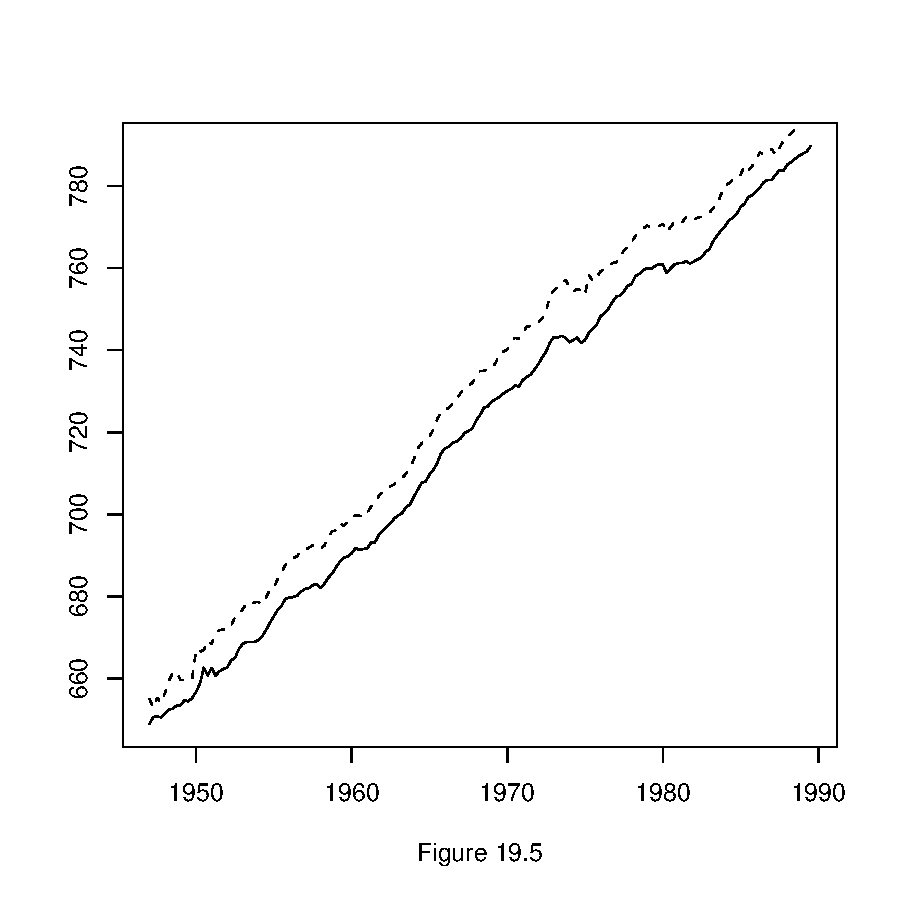
\includegraphics{Companion-075}
\subsection{Estimating the Cointegrating Vector}
Page 598 shows an example of the Phillips Ouliaris Hansen procedure for estimating a cointegrating vector.
\begin{Schunk}
\begin{Sinput}
 poh.cointegration.lm <- lm(p ~ 1 + ner + pstar, ppp.data)
 poh.residual.lms <- summary(lm(u ~ 0 + u_1, data.frame(u = poh.cointegration.lm$residuals[-1], 
+     u_1 = poh.cointegration.lm$residuals[-length(poh.cointegration.lm$residuals)])))
 POH.results <- Phillips.Perron(T = length(poh.residual.lms$residuals), 
+     rho = poh.residual.lms$coefficients[["u_1", "Estimate"]], 
+     sigma.rho = poh.residual.lms$coefficients[["u_1", "Std. Error"]], 
+     s = poh.residual.lms$sigma, lambda.hat.sq = as.numeric(Newey.West(poh.residual.lms$residuals %o% 
+         1, 12)), gamma0 = mean(poh.residual.lms$residuals^2))
 print(summary(poh.cointegration.lm)$coefficients)
\end{Sinput}
\begin{Soutput}
              Estimate  Std. Error   t value      Pr(>|t|)
(Intercept) 2.71231296 0.367695493  7.376519  4.298888e-12
ner         0.05134848 0.012045369  4.262923  3.114337e-05
pstar       0.53004097 0.006708385 79.011705 3.148050e-152
\end{Soutput}
\begin{Sinput}
 print(poh.residual.lms$coefficients)
\end{Sinput}
\begin{Soutput}
     Estimate Std. Error  t value     Pr(>|t|)
u_1 0.9833108 0.01171956 83.90338 7.71577e-158
\end{Soutput}
\begin{Sinput}
 print(POH.results)
\end{Sinput}
\begin{Soutput}
$T
[1] 201

$rho
[1] 0.9833108

$sigma.rho
[1] 0.01171956

$s.sq
[1] 0.1630028

$lambda.hat.sq
[1] 0.4082242

$gamma0
[1] 0.1621919

$rho.stat
[1] -7.542281

$t.stat
[1] -2.020981
\end{Soutput}
\end{Schunk}
A second example performs a similar analysis on quarterly US consumption and income data from 1947Q1 to 1989Q4.
\begin{Schunk}
\begin{Sinput}
 data(coninc, package = "Ham94")
 selection <- subset(coninc, Quarter >= "1947-01-01" & Quarter <= 
+     "1989-07-01")
 coninc.data <- data.frame(Quarter = selection$Quarter, cons = 100 * 
+     log(selection$GC82), inc = 100 * log(selection$GYD82))
\end{Sinput}
\end{Schunk}
\includegraphics{Companion-078}
Test individual series for unit root status using Dickey Fuller.
\begin{Schunk}
\begin{Sinput}
 for (series.name in c("inc", "cons")) do.DF(series = coninc.data[[series.name]], 
+     lag = 6)
\end{Sinput}
\begin{Soutput}
                Estimate  Std. Error     t value     Pr(>|t|)
(Intercept) 20.336729221 15.04162460  1.35203010 1.783352e-01
yt_1         0.970584904  0.02306293 42.08419931 1.029200e-86
tt           0.023796844  0.01985318  1.19864142 2.324968e-01
delta.yt_1  -0.006528755  0.08092856 -0.08067307 9.358060e-01
delta.yt_2  -0.035846316  0.08025935 -0.44663103 6.557649e-01
delta.yt_3   0.102128545  0.07758036  1.31642276 1.899755e-01
delta.yt_4  -0.187536343  0.07699406 -2.43572477 1.599577e-02
delta.yt_5  -0.037187883  0.07813842 -0.47592314 6.347992e-01
delta.yt_6   0.027855951  0.07662877  0.36351818 7.167132e-01
$T
[1] 164

$rho
[1] 0.970585

$sigma.rho
[1] 0.02306293

$zeta
  delta.yt_1   delta.yt_2   delta.yt_3   delta.yt_4   delta.yt_5   delta.yt_6 
-0.006528755 -0.035846316  0.102128545 -0.187536343 -0.037187883  0.027855951 

$rho.stat
[1] -4.242382

$t.stat
[1] -1.275428

[1] 1.132134
               Estimate  Std. Error    t value     Pr(>|t|)
(Intercept) 29.46860131 15.19248322  1.9396830 5.423391e-02
yt_1         0.95552168  0.02360001 40.4881863 2.508405e-84
tt           0.03721088  0.02006161  1.8548306 6.552012e-02
delta.yt_1   0.03624864  0.07979877  0.4542506 6.502840e-01
delta.yt_2   0.25964745  0.07935028  3.2721680 1.315743e-03
delta.yt_3   0.06273192  0.08172798  0.7675697 4.439106e-01
delta.yt_4  -0.05234112  0.08122252 -0.6444163 5.202580e-01
delta.yt_5  -0.04791625  0.07956524 -0.6022260 5.479037e-01
delta.yt_6  -0.06782142  0.07919698 -0.8563637 3.931186e-01
$T
[1] 164

$rho
[1] 0.9555217

$sigma.rho
[1] 0.02360001

$zeta
 delta.yt_1  delta.yt_2  delta.yt_3  delta.yt_4  delta.yt_5  delta.yt_6 
 0.03624864  0.25964745  0.06273192 -0.05234112 -0.04791625 -0.06782142 

$rho.stat
[1] -9.011597

$t.stat
[1] -1.884673

[1] 1.858290
\end{Soutput}
\end{Schunk}
Estimate cointegration vector, then check for unit root status of the residual using Phillips Perron.
\begin{Schunk}
\begin{Sinput}
 poh.cointegration.lm <- lm(cons ~ 1 + inc, coninc.data)
 poh.residual.lms <- summary(lm(u ~ 0 + u_1, data.frame(u = poh.cointegration.lm$residuals[-1], 
+     u_1 = poh.cointegration.lm$residuals[-length(poh.cointegration.lm$residuals)])))
 POH.results <- Phillips.Perron(T = length(poh.residual.lms$residuals), 
+     rho = poh.residual.lms$coefficients[["u_1", "Estimate"]], 
+     sigma.rho = poh.residual.lms$coefficients[["u_1", "Std. Error"]], 
+     s = poh.residual.lms$sigma, lambda.hat.sq = as.numeric(Newey.West(poh.residual.lms$residuals %o% 
+         1, 6)), gamma0 = mean(poh.residual.lms$residuals^2))
 print(summary(poh.cointegration.lm)$coefficients)
\end{Sinput}
\begin{Soutput}
             Estimate  Std. Error     t value      Pr(>|t|)
(Intercept) 0.6675807 2.350348907   0.2840347  7.767315e-01
inc         0.9864943 0.003217444 306.6080542 5.567137e-234
\end{Soutput}
\begin{Sinput}
 print(poh.residual.lms$coefficients)
\end{Sinput}
\begin{Soutput}
     Estimate Std. Error  t value     Pr(>|t|)
u_1 0.7818542 0.04788553 16.32757 1.402076e-36
\end{Soutput}
\begin{Sinput}
 print(POH.results)
\end{Sinput}
\begin{Soutput}
$T
[1] 170

$rho
[1] 0.7818542

$sigma.rho
[1] 0.04788553

$s.sq
[1] 1.22395

$lambda.hat.sq
[1] 1.030594

$gamma0
[1] 1.216750

$rho.stat
[1] -32.04525

$t.stat
[1] -4.27529
\end{Soutput}
\end{Schunk}
\subsection{Testing Hypotheses About the Cointegrating Vector}
Page 608-612 illustrate a technique that uses leads and lags to produce a stationary
vector for hypothesis testing.
\begin{Schunk}
\begin{Sinput}
 T <- length(coninc.data$Quarter)
 lead.lag.data <- list(ct = coninc.data$cons[c(-1:-5, -((T - 3):T))], 
+     yt = coninc.data$inc[c(-1:-5, -((T - 3):T))], delta.yt = diff(coninc.data$inc[c(-1:-4, 
+         -((T - 3):T))]), delta.yt_ = embed(diff(coninc.data$inc[-((T - 
+         4):T)]), 4), delta.yt. = embed(diff(coninc.data$inc[-1:-5])[(T - 
+         6):1], 4)[(T - 9):1, ], tt = 6:(T - 4))
\end{Sinput}
\end{Schunk}
The regression is estimated with both no trend and trend, and the corrected t-stat is calculated.
\begin{Schunk}
\begin{Sinput}
 no.trend.lm <- lm(ct ~ 1 + yt + delta.yt. + delta.yt + delta.yt_, 
+     lead.lag.data)
 trend.lm <- lm(ct ~ 1 + yt + tt + delta.yt. + delta.yt + delta.yt_, 
+     lead.lag.data)
 for (model in list(no.trend.lm, trend.lm)) {
+     lags <- 2
+     cms <- summary(model)
+     T <- length(cms$residuals)
+     cfs <- cms$coefficients
+     t.rho <- (cfs[["yt", "Estimate"]] - 1)/cfs[["yt", "Std. Error"]]
+     rms <- summary(lm(u ~ 0 + u_, list(u = cms$residuals[-c(1:lags)], 
+         u_ = embed(cms$residuals[-T], lags))))
+     sigma1.hat.sq <- mean(rms$residuals^2)
+     lambda.11 <- sigma1.hat.sq^0.5/(1 - sum(rms$coefficients[paste("u_", 
+         1:lags, sep = ""), "Estimate"]))
+     t.a <- t.rho * cms$sigma/lambda.11
+     print(cfs)
+     print(rms$coefficients)
+     print(T)
+     print(cms$sigma)
+     print(t.rho)
+     print(sigma1.hat.sq)
+     print(lambda.11)
+     print(t.a)
+ }
\end{Sinput}
\begin{Soutput}
               Estimate  Std. Error     t value      Pr(>|t|)
(Intercept) -4.51922906 2.340224673  -1.9311091  5.534290e-02
yt           0.99215853 0.003063317 323.8837231 1.617626e-216
delta.yt.1   0.48592391 0.115704789   4.1996871  4.551158e-05
delta.yt.2   0.26411856 0.114892015   2.2988418  2.288546e-02
delta.yt.3   0.28614193 0.115594505   2.4753939  1.441397e-02
delta.yt.4   0.14530952 0.118799555   1.2231487  2.231790e-01
delta.yt    -0.24036007 0.117415901  -2.0470828  4.238356e-02
delta.yt_1  -0.01101143 0.113899420  -0.0966768  9.231113e-01
delta.yt_2   0.06969114 0.111505773   0.6250003  5.329142e-01
delta.yt_3   0.04055551 0.111155199   0.3648548  7.157303e-01
delta.yt_4   0.02150153 0.110083985   0.1953193  8.454056e-01
     Estimate Std. Error  t value     Pr(>|t|)
u_1 0.7179687 0.07722647 9.296924 1.127578e-16
u_2 0.2057401 0.07684783 2.677241 8.207043e-03
[1] 162
[1] 1.516006
[1] -2.559799
[1] 0.3809180
[1] 8.089864
[1] -0.4796954
                Estimate  Std. Error    t value     Pr(>|t|)
(Intercept) 198.87166510 15.01478288 13.2450577 5.215628e-27
yt            0.68117915  0.02292367 29.7150967 9.919458e-65
tt            0.26895671  0.01974617 13.6207037 5.213974e-28
delta.yt.1    0.40061828  0.07787309  5.1445023 8.270282e-07
delta.yt.2    0.15407283  0.07749787  1.9880910 4.862147e-02
delta.yt.3    0.16559666  0.07805023  2.1216678 3.550904e-02
delta.yt.4    0.02782397  0.08016237  0.3470952 7.290063e-01
delta.yt     -0.05124600  0.07998305 -0.6407108 5.226882e-01
delta.yt_1    0.12737594  0.07708222  1.6524685 1.005308e-01
delta.yt_2    0.23116996  0.07573754  3.0522506 2.687346e-03
delta.yt_3    0.20472613  0.07553655  2.7102923 7.505953e-03
delta.yt_4    0.18997478  0.07487875  2.5370986 1.219919e-02
     Estimate Std. Error  t value     Pr(>|t|)
u_1 0.6871713 0.07786238 8.825460 1.937474e-15
u_2 0.1291820 0.07666487 1.685022 9.395837e-02
[1] 162
[1] 1.017016
[1] -13.90793
[1] 0.3439489
[1] 3.193478
[1] -4.429212
\end{Soutput}
\end{Schunk}

\section{Full-Information Maximum Likelihood Analysis of Cointegrated Systems}
\subsection{An Application of the Johansen Approach to the PPP data}
Section 20.3 reanalyzes the data used in Chapter 19 using the FIML approach. 
\begin{Schunk}
\begin{Sinput}
 data(ppp, package = "Ham94")
 selection <- subset(ppp, Month >= "1973-01-01" & Month <= "1989-10-01")
 ppp.data <- data.frame(pstar = 100 * log(selection$PC6IT/selection$PC6IT[[1]]), 
+     p = 100 * log(selection$PZUNEW/selection$PZUNEW[[1]]), ner = -100 * 
+         log(selection$EXRITL/selection$EXRITL[[1]]))
 y <- as.matrix(ppp.data)
\end{Sinput}
\end{Schunk}
First conduct the auxiliary regressions.  Given that the right hand sides consists of lagged values of the changes in y
for both [20.2.4] and [20.2.5], construct a regression with both lagged y and lagged changes of y as left hand side.
\begin{Schunk}
\begin{Sinput}
 delta.y <- diff(y)
 lags <- 12
 X <- embed(delta.y[-dim(delta.y)[[1]], ], lags)
 T <- dim(X)[[1]]
 n <- dim(y)[[2]]
 lhs <- cbind(delta.y[-1:(-lags), ], y[c(-1:-lags, -(T + lags + 
+     1)), ])
 aux.lm <- lm(lhs ~ 1 + X, list(lhs = lhs, X = X))
 uv <- sapply(summary(aux.lm), FUN = function(x) {
+     x$residuals
+ })
 u <- uv[, 1:n]
 v <- uv[, (n + 1):(2 * n)]
\end{Sinput}
\end{Schunk}
Now calculate the canonical correlations according to [20.2.6], [20.2.7], [20.2.8],
and calculate eigenvalues according to [20.2.9], and log likelihood as in [20.2.10].
Note that u is T rows by n columns
so that ut is the t-th row of matrix u, so only a single inner product, rather than sum of outer products, is needed.
\begin{Schunk}
\begin{Sinput}
 SigmaUU <- 1/T * t(u) %*% u
 SigmaVV <- 1/T * t(v) %*% v
 SigmaUV <- 1/T * t(u) %*% v
 eigen.results <- eigen(solve(SigmaVV) %*% t(SigmaUV) %*% solve(SigmaUU) %*% 
+     SigmaUV)
 lambda <- eigen.results$values
 LRT <- -T * sum(log(1 - lambda))
 print(SigmaUU)
\end{Sinput}
\begin{Soutput}
               Response pstar  Response p Response ner
Response pstar     0.17931504  0.01531134   0.02715177
Response p         0.01531134  0.04341512  -0.03267373
Response ner       0.02715177 -0.03267373   4.60842626
\end{Soutput}
\begin{Sinput}
 print(SigmaVV)
\end{Sinput}
\begin{Soutput}
               Response pstar Response p Response ner
Response pstar      1503.5545   794.7041    -697.4981
Response p           794.7041   421.5535    -365.1883
Response ner        -697.4981  -365.1883     414.1322
\end{Soutput}
\begin{Sinput}
 print(SigmaUV)
\end{Sinput}
\begin{Soutput}
               Response pstar Response p Response ner
Response pstar     -3.5787320 -1.7958934    1.5095381
Response p         -0.8602478 -0.4969721    0.5243431
Response ner       -3.1461173 -2.0636489   -2.2685853
\end{Soutput}
\begin{Sinput}
 print(lambda)
\end{Sinput}
\begin{Soutput}
[1] 0.12002316 0.05077020 0.03174158
\end{Soutput}
\begin{Sinput}
 print(T * log(1 - lambda))
\end{Sinput}
\begin{Soutput}
[1] -24.165480  -9.847724  -6.096434
\end{Soutput}
\begin{Sinput}
 print(LRT)
\end{Sinput}
\begin{Soutput}
[1] 40.10964
\end{Soutput}
\end{Schunk}
Finally following page 648, calculate the first cointegrating vector normalized as in [20.3.9], and also
normalized to have unity for the first coefficient.
\begin{Schunk}
\begin{Sinput}
 ahat1 <- eigen.results$vectors[, 1]
 ahat1.tilde <- ahat1/sqrt(t(ahat1) %*% SigmaVV %*% ahat1)
 ahat1.normal <- ahat1/ahat1[[1]]
 print(ahat1)
\end{Sinput}
\begin{Soutput}
[1] -0.48885151  0.87144476 -0.04010268
\end{Soutput}
\begin{Sinput}
 print(ahat1.tilde)
\end{Sinput}
\begin{Soutput}
[1] -0.44788450  0.79841545 -0.03674197
\end{Soutput}
\begin{Sinput}
 print(ahat1.normal)
\end{Sinput}
\begin{Soutput}
[1]  1.00000000 -1.78263694  0.08203448
\end{Soutput}
\end{Schunk}
\subsection{Likelihood Ratio Tests on the Cointegration Vector}
Page 649 shows how to conduct hypothesis tests on the cointegration vector.  The follow code implements
[20.3.10] - [20.3.14] and subsequent calculations.
\begin{Schunk}
\begin{Sinput}
 D = cbind(c(1, 0, 0), c(0, 0, 1))
 SigmaVV.tilde <- t(D) %*% SigmaVV %*% D
 SigmaUV.tilde <- SigmaUV %*% D
 eigen.results <- eigen(solve(SigmaVV.tilde) %*% t(SigmaUV.tilde) %*% 
+     solve(SigmaUU) %*% SigmaUV.tilde)
 lambda.tilde <- eigen.results$values
 h <- 1
 LRT <- -T * sum(log(1 - lambda[1:h])) + T * sum(log(1 - lambda.tilde[1:h]))
 ahat1.normal.tilde <- eigen.results$vectors[, 1]/eigen.results$vectors[, 
+     1][[1]]
 print(SigmaVV.tilde)
\end{Sinput}
\begin{Soutput}
          [,1]      [,2]
[1,] 1503.5545 -697.4981
[2,] -697.4981  414.1322
\end{Soutput}
\begin{Sinput}
 print(SigmaUV.tilde)
\end{Sinput}
\begin{Soutput}
                     [,1]       [,2]
Response pstar -3.5787320  1.5095381
Response p     -0.8602478  0.5243431
Response ner   -3.1461173 -2.2685853
\end{Soutput}
\begin{Sinput}
 print(lambda.tilde)
\end{Sinput}
\begin{Soutput}
[1] 0.05828948 0.03295258
\end{Soutput}
\begin{Sinput}
 print(T * log(1 - lambda.tilde))
\end{Sinput}
\begin{Soutput}
[1] -11.350839  -6.332964
\end{Soutput}
\begin{Sinput}
 print(LRT)
\end{Sinput}
\begin{Soutput}
[1] 12.81464
\end{Soutput}
\begin{Sinput}
 print(ahat1.normal.tilde)
\end{Sinput}
\begin{Soutput}
[1] 1.000000 1.012463
\end{Soutput}
\end{Schunk}
Page 650 shows a second example.
\begin{Schunk}
\begin{Sinput}
 h <- 1
 D = c(1, -1, -1) %o% 1
 SigmaVV.tilde <- t(D) %*% SigmaVV %*% D
 SigmaUV.tilde <- SigmaUV %*% D
 eigen.results <- eigen(solve(SigmaVV.tilde) %*% t(SigmaUV.tilde) %*% 
+     solve(SigmaUU) %*% SigmaUV.tilde)
 lambda.tilde <- eigen.results$values
 LRT <- -T * sum(log(1 - lambda[1:h])) + T * sum(log(1 - lambda.tilde[1:h]))
 print(SigmaVV.tilde)
\end{Sinput}
\begin{Soutput}
         [,1]
[1,] 1414.452
\end{Soutput}
\begin{Sinput}
 print(SigmaUV.tilde)
\end{Sinput}
\begin{Soutput}
                     [,1]
Response pstar -3.2923768
Response p     -0.8876187
Response ner    1.1861170
\end{Soutput}
\begin{Sinput}
 print(lambda.tilde)
\end{Sinput}
\begin{Soutput}
[1] 0.04912925
\end{Soutput}
\begin{Sinput}
 print(T * log(1 - lambda.tilde))
\end{Sinput}
\begin{Soutput}
[1] -9.521278
\end{Soutput}
\begin{Sinput}
 print(LRT)
\end{Sinput}
\begin{Soutput}
[1] 14.64420
\end{Soutput}
\end{Schunk}
\section{Time Series Models of Heteroskedasticity}
\subsection{Preamble}
Page 658 and forward provide examples of ARCH models.  Several utility functions are needed for these examples.
The function "arch.fitted.values" calculates the value of ht given the conditional information set YT and
a parameter vector THETA as described on page 660, [21.1.17] to [21.1.20].
\begin{Schunk}
\begin{Sinput}
 arch.fitted.values <- function(THETA, YT) {
+     alpha <- THETA[grep("alpha.*", names(THETA))]
+     beta <- THETA[grep("beta.*", names(THETA))]
+     zeta <- THETA["zeta"]
+     m <- length(alpha)
+     h <- rep(as.vector(zeta), m)
+     u <- YT$y - YT$x %*% beta
+     indices <- (m + 1):length(YT$y)
+     z <- array(0, c(length(indices), 1 + m))
+     for (tt in indices) h[tt] <- t(c(zeta, alpha)) %*% c(1, u[(tt - 
+         1):(tt - m)]^2)
+     list(u = u, h = h)
+ }
\end{Sinput}
\end{Schunk}
Function "arch.standard.errors" calculates values for standard errors according to the description on page 663,
particularly equations [21.1.25], and also using [21.1.21] for the estimate of the outer product estimate of the
information matrix.
\begin{Schunk}
\begin{Sinput}
 arch.standard.errors <- function(THETA, YT) {
+     x <- YT$x
+     y <- YT$y
+     k <- dim(x)[[2]]
+     alpha <- THETA[grep("alpha.*", names(THETA))]
+     zeta <- THETA["zeta"]
+     m <- length(alpha)
+     T <- length(y) - m
+     a <- k + 1 + m
+     fv <- arch.fitted.values(THETA, YT)
+     h <- fv$h
+     u2 <- fv$u^2
+     S <- array(0, c(a, a))
+     D <- array(0, c(a, a))
+     for (tt in (m + 1):length(y)) {
+         temp <- c(t(alpha) %*% ((u2[(tt - 1):(tt - m)] %o% rep(1, 
+             k)) * x[(tt - 1):(tt - m), ]), c(1, u[(tt - 1):(tt - 
+             m)]^2))
+         st <- (u2[tt] - h[tt])/(2 * h[tt]^2) * temp + c(u2[tt]/h[tt] * 
+             x[tt, ], rep(0, a - k))
+         S <- S + 1/T * st %*% t(st)
+         D <- D + 1/T * (1/(2 * h[tt]^2) * temp %*% t(temp) + 
+             rbind(cbind(1/h[tt] * x[tt, ] %*% t(x[tt, ]), array(0, 
+                 c(k, a - k))), array(0, c(a - k, a))))
+     }
+     diag(1/T * solve(D) %*% S %*% solve(D))^0.5
+ }
\end{Sinput}
\end{Schunk}
The following two helper functions calculate the likelihood values under different distributional assumptions.
The normal likelihood is calculated according to [21.1.20], the scaled t according to [21.1.24].
\begin{Schunk}
\begin{Sinput}
 arch.normal <- function(THETA, YT) {
+     fv <- arch.fitted.values(THETA, YT)
+     m <- length(THETA[grep("alpha.*", names(THETA))])
+     h <- fv$h[-1:-m]
+     u <- fv$u[-1:-m]
+     -1/2 * (length(h) * log(2 * pi) - sum(log(h)) - sum(u^2/h))
+ }
 arch.scaled.t <- function(THETA, YT) {
+     fv <- arch.fitted.values(THETA, YT)
+     m <- length(THETA[grep("alpha.*", names(THETA))])
+     h <- fv$h[-1:-m]
+     u <- fv$u[-1:-m]
+     nu <- THETA[grep("nu", names(THETA))]
+     result <- length(h) * log(gamma((nu + 1)/2)/(sqrt(pi) * gamma(nu/2)) * 
+         (nu - 2)^-0.5) - 1/2 * sum(log(h)) - (nu + 1)/2 * sum(log(1 + 
+         u^2/(h * (nu - 2))))
+ }
\end{Sinput}
\end{Schunk}
GMM estimates are calculated according to the recipe in Chapter 14, notably
equations [14.1.7] and [14.1.10].  Functions h and S are specified
by the caller.
\begin{Schunk}
\begin{Sinput}
 GMM.estimates <- function(YT, h, THETA, S) {
+     g <- function(YT, THETA) {
+         apply(X = apply(X = YT, MARGIN = 1, FUN = h, THETA = THETA), 
+             MARGIN = 1, FUN = mean)
+     }
+     objective <- function(THETA, YT, W) {
+         g.value <- g(YT, THETA)
+         as.numeric(t(g.value) %*% W %*% g.value)
+     }
+     r <- length(h(YT[1, ], THETA))
+     a <- length(THETA)
+     stage.1.results <- optim(par = THETA, fn = objective, gr = NULL, 
+         YT = YT, W = diag(r))
+     temp <- t(apply(X = YT, MARGIN = 1, FUN = h, THETA = stage.1.results$par))
+     ST <- S(temp)
+     stage.2.results <- optim(par = stage.1.results$par, fn = objective, 
+         gr = NULL, YT = YT, W = solve(ST))
+     list(stage.1.results = stage.1.results, stage.2.results = stage.2.results)
+ }
\end{Sinput}
\end{Schunk}
\subsection{Application of ARCH Models to US Fed Funds Data}
The dataset for these examples is the US Fed Funds Rate, monthly between Jan 1955 and December 2000,
shown below.
\begin{Schunk}
\begin{Sinput}
 data(fedfunds, package = "Ham94")
 selection <- subset(fedfunds, Month >= "1955-01-01" & Month <= 
+     "2000-12-01")
 y <- selection$FFED
\end{Sinput}
\end{Schunk}
\includegraphics{Companion-094}
A first step is to characterize the autocorrelation structure of the squared residuals.  These two regressions
show that a second order AR process seems to fit the data pretty well.
\begin{Schunk}
\begin{Sinput}
 y.lm <- lm(y ~ 1 + y_1, list(y = y[-1], y_1 = y[-length(y)]))
 u <- y.lm$residuals
 u2.lm <- lm(u2 ~ 1 + u2_lag, list(u2 = u[-1:-4]^2, u2_lag = embed(u[-length(u)]^2, 
+     4)))
 F34 <- Wald.F.Test(R = cbind(rep(0, 2) %o% rep(0, 3), diag(2)), 
+     b = u2.lm$coefficients, r = c(0, 0), s2 = summary(u2.lm)$sigma^2, 
+     XtX_1 = summary(u2.lm)$cov.unscaled)
 F34.sig <- 1 - pf(F34, 2, length(u2.lm$residuals) - u2.lm$rank)
 F234 <- Wald.F.Test(R = cbind(rep(0, 3) %o% rep(0, 2), diag(3)), 
+     b = u2.lm$coefficients, r = c(0, 0, 0), s2 = summary(u2.lm)$sigma^2, 
+     XtX_1 = summary(u2.lm)$cov.unscaled)
 F234.sig <- 1 - pf(F234, 3, length(u2.lm$residuals) - u2.lm$rank)
 accept.arch <- pchisq(length(u2.lm$residuals) * summary(u2.lm)$r.squared, 
+     4)
 print(F34)
\end{Sinput}
\begin{Soutput}
[1] 0.8225742
\end{Soutput}
\begin{Sinput}
 print(F34.sig)
\end{Sinput}
\begin{Soutput}
[1] 0.439847
\end{Soutput}
\begin{Sinput}
 print(F234)
\end{Sinput}
\begin{Soutput}
[1] 11.88167
\end{Soutput}
\begin{Sinput}
 print(F234.sig)
\end{Sinput}
\begin{Soutput}
[1] 1.513714e-07
\end{Soutput}
\begin{Sinput}
 print(accept.arch)
\end{Sinput}
\begin{Soutput}
[1] 1
\end{Soutput}
\end{Schunk}
Next we use a maximum likelihood estimation to estimate the parameters for the second
order equation assuming normal errors.
\begin{Schunk}
\begin{Sinput}
 YT <- list(y = y[-1], x = cbind(rep(1, length(y) - 1), y[-length(y)]))
 THETA <- c(beta = y.lm$coefficients, zeta = var(y.lm$residuals), 
+     alpha = c(0.1, 0.1))
 optimizer.results <- optim(par = THETA, fn = arch.normal, gr = NULL, 
+     YT = YT)
 print(optimizer.results$par)
\end{Sinput}
\begin{Soutput}
beta.(Intercept)         beta.y_1             zeta           alpha1 
      0.25226382       0.94858488       0.02734929       0.95530391 
          alpha2 
      0.29858866 
\end{Soutput}
\begin{Sinput}
 se <- arch.standard.errors(optimizer.results$par, YT)
 print(se)
\end{Sinput}
\begin{Soutput}
[1] 0.048395622 0.010418563 0.004969357 0.108784800 0.082012310
\end{Soutput}
\end{Schunk}
Now use GMM to estimate the same parameters following page 664.  The initial values
for the regression coefficients are derived from the (homoskedastic) regression above,
as is the presample variance.  The estimator for S assumes no correlation at leads and lags.
\begin{Schunk}
\begin{Sinput}
 h <- function(wt, THETA) {
+     beta <- THETA[grep("beta.*", names(THETA))]
+     zeta <- THETA["zeta"]
+     alpha <- THETA[grep("alpha.*", names(THETA))]
+     m <- length(alpha)
+     k <- length(beta)
+     yt <- wt[grep("yt.*", names(wt))]
+     xt <- wt[grep("xt.*", names(wt))]
+     ylagt <- wt[grep("ylagt.*", names(wt))]
+     xlagt <- t(array(wt[grep("xlagt.*", names(wt))], c(k, m)))
+     ut <- yt - t(xt) %*% beta
+     zt <- c(1, (ylagt - t(xlagt) %*% beta)^2)
+     c(ut * xt, (ut^2 - t(zt) %*% c(zeta, alpha)) * zt)
+ }
 S.estimator <- function(ht) {
+     1/dim(ht)[[1]] * t(ht) %*% ht
+ }
 THETA <- c(beta = y.lm$coefficients, zeta = var(y.lm$residuals), 
+     alpha = c(0.1, 0.1))
 m <- length(THETA[grep("alpha.*", names(THETA))])
 T <- length(YT$y) - m
 w <- as.matrix(data.frame(yt = YT$y[-1:-m], xt = YT$x[-1:-m, 
+     ], ylagt = embed(YT$y[-(T + m)], m), xlagt = embed(YT$x[-(T + 
+     m), ], m)))
 estimates <- GMM.estimates(YT = w, h = h, THETA = THETA, S.estimator)
 print(estimates$stage.1.results$par)
\end{Sinput}
\begin{Soutput}
beta.(Intercept)         beta.y_1             zeta           alpha1 
      0.05788674       0.98955937       0.32491651       0.01073606 
          alpha2 
      0.02105476 
\end{Soutput}
\begin{Sinput}
 print(estimates$stage.2.results$par)
\end{Sinput}
\begin{Soutput}
beta.(Intercept)         beta.y_1             zeta           alpha1 
      0.02579794       0.99791508      -0.17911928       0.01239927 
          alpha2 
      0.07770754 
\end{Soutput}
\end{Schunk}
\subsection{R Facilities For GARCH models}
TBD
\section{Modeling Time Series with Changes in Regime}
\subsection{Modeling Changes in Regime}
Page 697 describes an example of the application of Markov switching models to US GNP from 1951Q1 to 1984Q4.
\begin{Schunk}
\begin{Sinput}
 data(gnpdata, package = "Ham94")
 selection <- subset(gnpdata, Quarter >= "1951-01-01" & Quarter <= 
+     "1984-04-01")
 d <- selection$Quarter[-1]
 g <- diff(100 * log(selection$GNP), lag = 1, differences = 1)
\end{Sinput}
\end{Schunk}

The actual implementation uses the technique of collapsing multi-period states into a single state, p691, p698.
During the maximum likelihood estimation process the state probabilities will change, but the layout of the matrix
is still the same.  The following code fragment precalculates the transition matrix structure with the five possible
values, then uses a separate 5 element lookup vector to populate it.
\begin{Schunk}
\begin{Sinput}
 nlags <- 4
 nstates <- 2^(nlags + 1)
 lagstate <- 1 + outer(1:nstates, 1:(nlags + 1), FUN = function(i, 
+     j) {
+     trunc((i - 1)/2^(nlags + 1 - j))%%2
+ })
 transit <- outer(X = 1:nstates, Y = 1:nstates, FUN = function(i, 
+     j) {
+     ((2 * lagstate[i, 1] + lagstate[j, 1] - 1) - 1) * (((i - 
+         1)%%(2^nlags)) == trunc((j - 1)/2)) + 1
+ })
\end{Sinput}
\end{Schunk}
The bulk of the work is done by the following function, based on the algorithm in section 22.4.
Ergodic probabilities are defined as on page 684, including equation [22.2.26].
The loop uses equations [22.4.24], [22.4.2], [22.4.5], [22.4.8], [22.4.7], [22.4.6] and [22.4.14].
\begin{Schunk}
\begin{Sinput}
 infer.regimes <- function(THETA, YT) {
+     phi <- THETA[grep("phi*", names(THETA))]
+     mu <- THETA[grep("mu*", names(THETA))]
+     sigma <- THETA["sigma"]
+     p11star <- THETA["p11star"]
+     p22star <- THETA["p22star"]
+     T <- length(YT)
+     tp <- c(0, p11star, 1 - p22star, 1 - p11star, p22star)
+     P <- array(tp[transit], c(nstates, nstates))
+     A <- rbind(diag(nstates) - P, rep(1, nstates))
+     ergodic.pi <- (solve(t(A) %*% A) %*% t(A))[, nstates + 1]
+     xi.t.t <- ergodic.pi %o% rep(1, nlags)
+     xi.t.t_1 <- cbind(xi.t.t, ergodic.pi)
+     log.likelihood <- 0
+     for (tt in (nlags + 1):T) {
+         residuals <- as.vector(((rep(1, nstates) %o% YT[tt:(tt - 
+             nlags)]) - array(mu[lagstate], c(nstates, nlags + 
+             1))) %*% c(1, -phi))
+         eta.t <- dnorm(residuals, mean = 0, sd = sigma)
+         fp <- eta.t * xi.t.t_1[, tt - 1]
+         fpt <- sum(fp)
+         xi.t.t <- cbind(xi.t.t, fp/fpt)
+         log.likelihood <- log.likelihood + log(fpt)
+         xi.t.t_1 <- cbind(xi.t.t_1, P %*% xi.t.t[, tt])
+     }
+     xi.t.T <- xi.t.t[, T] %o% 1
+     for (tt in (T - 1):1) xi.t.T <- cbind(xi.t.t[, tt] * (t(P) %*% 
+         (xi.t.T[, 1]/xi.t.t_1[, tt + 1])), xi.t.T)
+     list(log.likelihood = log.likelihood, xi.t.t = xi.t.t, xi.t.T = xi.t.T)
+ }
\end{Sinput}
\end{Schunk}
Initial values of the parameters for transition probabilities are set from historical averages.
The phi and sigma values are obtained from a (non-state) regression of change in GDP on 4 of its own lags.
\begin{Schunk}
\begin{Sinput}
 g.lm <- lm(g ~ 1 + g_lag, list(g = g[-1:-nlags], g_lag = embed(g[-length(g)], 
+     nlags)))
 THETA <- c(p11star = 0.85, p22star = 0.7, mu = c(1, 0), phi = as.vector(g.lm$coefficients[1 + 
+     (1:nlags)]), sigma = summary(g.lm)$sigma)
\end{Sinput}
\end{Schunk}
Now we are in a position to optimize, then calculated the smoothed probabilities from the
optimal parameters. 
\begin{Schunk}
\begin{Sinput}
 objective <- function(THETA, YT) {
+     -infer.regimes(THETA, YT)$log.likelihood
+ }
 optimizer.results <- optim(par = THETA, hessian = TRUE, fn = objective, 
+     gr = NULL, YT = g)
 se <- diag(solve(optimizer.results$hessian))^0.5
 print(optimizer.results$par)
\end{Sinput}
\begin{Soutput}
     p11star      p22star          mu1          mu2         phi1         phi2 
 0.869651020  0.657920015  1.095327317 -0.198544833  0.311107386  0.092829514 
        phi3         phi4        sigma 
-0.125038400 -0.007166502  0.872625052 
\end{Soutput}
\begin{Sinput}
 print(se)
\end{Sinput}
\begin{Soutput}
   p11star    p22star        mu1        mu2       phi1       phi2       phi3 
0.13323951 0.04404274 0.23169921        NaN 0.08762475 0.10748667 0.09374541 
      phi4      sigma 
0.08826466        NaN 
\end{Soutput}
\begin{Sinput}
 regimes <- infer.regimes(optimizer.results$par, g)
 recession.probability <- as.vector((1:nstates > nstates/2) %*% 
+     regimes$xi.t.t)
 smoothed.recession.probability <- as.vector((1:nstates > nstates/2) %*% 
+     regimes$xi.t.T)
\end{Sinput}
\end{Schunk}
The results are shown below.
\begin{center}
\includegraphics{Companion-103}
\end{center}

\end{document}
